% ZhCvGo15.tex      pdflatex ZhCvGo15

% Diffuse globally, compute locally: a cyclist tale
% Tingnan Zhang, Daniel I. Goldman and Predrag Cvitanovi\'c

                  %%   logical setup, no need to edit %%%%%%%%%%
                  \newif\ifpaper \paperfalse \newif\ifPDF \PDFtrue %%
                  \newif\ifboyscout %%
                  \boyscouttrue %% commented, WWW/drafts %%
%%%% Toggle between draft and public versions
% \boyscoutfalse % public, for hyperlinked pdf

% Predrag                       2015-11-19
% Tingnan                       2015-11-

        \ifboyscout
\documentclass[aps,pre,
                showpacs,
                twocolumn,
                %preprint,      %uncomment for double spacing
                groupedaddress,
                floatfix]{revtex4-1}
        \else
\documentclass[pre,aps,
                twocolumn,
                showpacs,
                superscriptaddress,
                groupedaddress,
                floatfix,
                hyperref]{revtex4-1}
        \fi
%   REVTeX 4 Version 4.1r August 2010
%   Phys. Rev. appearance, change preprint to twocolumn.  Choose pra,
%   prb, prc, prd, pre, prl, prstab for journal Add
%   'draft' option to mark overfull boxes with black boxes Add
%   'showpacs' option to make PACS codes appear Add 'showkeys' option
%   to make keywords appear
% Use the \preprint command to place your local institutional report
% number in the upper righthand corner of the title page in preprint
% mode.  Multiple \preprint commands are allowed.  Use the
% 'preprintnumbers' class option to override journal defaults to
% display numbers if necessary \preprint{}

%%%%%%%%%%%%%%%%%%%%%%%%%%%%%%%%%%%%%%%%%%%%%%%%%%%%%%%%%%%%%%
% GitHub cvitanov/reducesymm/inputs/setupSveZha.tex
% $Author$ $Date$
% Predrag                                       2014-04-18

                        %% logical setup, no need to edit %%%%%%%%%%
                        \newif\ifpaper \newif\ifPDF               %%
                        \newif\ifOUP \newif\ifboyscout            %%
                        \newif\ifdasbuch \newif\iftoCB            %%
                        \newif\ifsolutions \newif\ifblog          %%
                        \blogtrue                                 %%
                        \boyscouttrue       %% commented, WWW/drafts %%
                        \dasbuchtrue %% DasBuch, not QFT lectures %%
                        \solutionstrue %% include solutions       %%
                        \paperfalse\PDFtrue %% hyperlinked        %%
                        \OUPfalse \toCBtrue      %% ChaosBook %%%%%%
%%%% Toggle between draft and non-draft versions
%    \boyscoutfalse        % public, for hyperlinked ChaosBook/projects

\usepackage[latin1]{inputenc}
\usepackage[T1]{fontenc}
\usepackage{times}
\usepackage[pdftex]{graphicx}
\usepackage{array}
\usepackage{verbatim}
\usepackage[pdftex,colorlinks]{hyperref}
\usepackage{amsmath}
\hypersetup{
   pdfauthor=Tingnan Zhang
   pdfkeywords=periodic orbits chaos deterministic diffusion
   pdftitle=periodic Lorentz gas: periodic orbits theory}

\graphicspath{{../Fig/}{../figs/}{figs/}}

% editsDasbuch.tex
% $Author$ $Date$

% Predrag extracted from DasBuch def.tex                   25jun2008

\ifboyscout %%%%%%%% DISPLAY COMMENTS IN THE TEXT %%%%%%%%%%%%%%%%%%%%
            %%%%%%%% turn on labeling of equations on margins %%%%%%%%
    % also search the text for lines starting with %%  to
    % locate various internal comments, recent edits etc.
    \typeout{============ COMMENTED =====}
  \newcommand{\PublicPrivate}[2]
    {\marginpar{\color{blue}$\Downarrow$\footnotesize PRIVATE}%
    {\color{blue}#2}%
    \marginpar{\color{blue}$\Uparrow$\footnotesize PRIVATE}}
  \newcommand{\PC}[1]{$\footnotemark\footnotetext{Predrag: #1}$}
  \newcommand{\PCedit}[1]{{\color{red}#1}}
  \newcommand{\JG}[1]{$\footnotemark\footnotetext{John G: #1}$}
  \newcommand{\JGedit}[1]{{\color{green}#1}}
  \newcommand{\DL}[1]{$\footnotemark\footnotetext{Domenico: #1}$}
  \newcommand{\DLedit}[1]{{\color{green}#1}}
  \newcommand{\ES}[1]{$\footnotemark\footnotetext{Vaggelis: #1}$}
  \newcommand{\ESedit}[1]{{\color{red}#1}}
  \newcommand{\JH}[1]{$\footnotemark\footnotetext{JH: #1}$}
  \newcommand{\JHedit}[1]{{\color{magenta}#1}}
  \newcommand{\RLD}[1]{$\footnotemark\footnotetext{Ruslan: #1}$}
  \newcommand{\RLDedit}[1]{{\color{magenta}#1}}
    %    \newcommand{\Preliminary}[1]
    %{\marginpar{\color{magenta}$\Downarrow$\footnotesize PRELIMINARY}%
    %{\color{magenta}#1}%
    %\marginpar{\color{magenta}$\Uparrow$\footnotesize PRELIMINARY}}
\else % drop comments
      % do not turn on labeling of equations on margins
  \typeout{============ UNCOMMENTED =====}
  \newcommand{\PublicPrivate}[2]{#1}
  \newcommand{\PC}[1]{}
  \newcommand{\PCedit}[1]{#1}
  \newcommand{\JG}[1]{}
  \newcommand{\JGedit}[1]{#1}
  \newcommand{\DL}[1]{}
  \newcommand{\DLedit}[1]{#1}
  \newcommand{\ES}[1]{}
  \newcommand{\ESedit}[1]{#1}
  \newcommand{\JH}[1]{}
  \newcommand{\JHedit}[1]{#1}
  \newcommand{\RLD}[1]{$}
  \newcommand{\RLDedit}[1]{#1}
    %  \newcommand{\Preliminary}[1]{}
\fi  %%%%%%%%%%%% END OF ON/OFF COMMENTS SWITCH %%%%%%%%%%%%%%%%%%%%
 %% editing comments, DasBuch style
% def.tex
% $Author$ $Date$

%%%%%%%%%%%%%%%%%%%%%%%%%%%%%%%%%%%%%%%%%%%%%%%%%%%%%%%%%%%%%%%%%%%%%%%%%
%% defines macros used throughout ChaosBook and related
%%%%%%%%%%%%%%%%%%%%%%%%%%%%%%%%%%%%%%%%%%%%%%%%%%%%%%%%%%%%%%%%%%%%%%%%%

%               Predrag          9oct2009
%               Predrag         12jun2008
%               Predrag         15dec2008
%               Predrag         29oct2005
%               Predrag         13jul2005
%               Predrag         24apr2005
%               Predrag         14feb2005
%               Predrag         22jan2005
%               Predrag         16nov2004
%               Predrag         13jun2004
%               Predrag          3may2004
%               Predrag         10apr2004
%               Predrag         21feb2004
%               Predrag          4oct2003
%               Predrag         30aug2003
%               Predrag         20jun2003
%               Predrag         17jan2003
%               Predrag          6dec2002
%               Predrag          7jul2002
%               Predrag         19nov2000
%               Ronnie          23sep2000
% Predrag disabled \basedirectory machine identifier    25aug2000
% Predrag created               30oct1994

\ifpaper % prepare for B&W paper printing:
       \newcommand{\href}[2]{{#2}}  % no hyperref
       \newcommand{\HREF}[2]{{#2}}
       \renewcommand{\color}[1]{}       % B&W
       \newcommand{\wwwcb}[1]{{\tt ChaosBook.org#1}}
       \newcommand{\wwwgt}{{\tt birtracks.eu}}
       \newcommand{\wwwQFT}[1]{{\tt ChaosBook.org/\-Field\-Theory#1}}
       \newcommand{\wwwcnsQFT}[1]{{\tt ChaosBook.org/\-Field\-Theory#1}}
       \newcommand{\weblink}[1]{{\tt #1}}
       \newcommand{\arXiv}[1]{ {\tt arXiv:#1}}
       \newcommand{\mpArc}[1]{{\tt \goodbreak mp\_arc~#1}}
\else % prepare hyperlinked pdf
        \newcommand{\wwwcb}[1]{       % keep homepage flexible:
                  {\tt \href{http://ChaosBook.org#1}
              {ChaosBook.org#1}}}
       \newcommand{\wwwgt}{{\tt \href{http://birtracks.eu}
              {birtracks.eu}}}
       \newcommand{\wwwQFT}[1]{
                  {\tt \href{http://ChaosBook.org/FieldTheory#1}
              {ChaosBook.org/\-Field\-Theory#1}}}
       \newcommand{\wwwcnsQFT}[1]{
                  {\tt \href{http://ChaosBook.org/FieldTheory#1}
              {ChaosBook.org/\-Field\-Theory#1}}}
       \newcommand{\weblink}[1]{{\tt \href{http://#1}{#1}}}
       \newcommand{\HREF}[2]{
              {\href{#1}{#2}}}
       \newcommand{\mpArc}[1]{
              {\tt \href{http://www.ma.utexas.edu/mp_arc-bin/mpa?yn=#1}
                   {\goodbreak mp\_arc~#1}}}
       \newcommand{\arXiv}[1]{
              {\tt \href{http://arXiv.org/abs/#1}{\goodbreak arXiv:#1}}}
\fi

%%%%%%%%%%%%%%%%%%%%%% QUOTATIONS %%%%%%%%%%%%%%%%%%%%%%%%%%%%%%%%%%%%%%
%
%  the learned/witty quotes at the chapter and section headings
%
\newsavebox{\bartName}
\newcommand{\bauthor}[1]{\sbox{\bartName}{\parbox{\textwidth}{\vspace*{0.8ex}
       %\hspace*{\fill}
       \hspace{2em}---\small\noindent #1}}}
\newenvironment{bartlett}{\hfill\begin{minipage}[t]{0.65\textwidth}\small}%
{\hspace*{\fill}\nolinebreak[1]\usebox{\bartName}\vspace*{1ex}\end{minipage}}
%
%  a quotation inserted into the text
%
\newenvironment{txtquote}{\begin{quotation} \small}{\end{quotation}}

\newcommand{\student}{Henri Roux}
%\newcommand{\student}{Jens J. Jensen}

%%%%%%%%%%%%%%%%%%%%%% INDEXING %%%%%%%%%%%%%%%%%%%%%%%%%%%%%%%%%%%%%%%%%
\newcommand{\indx}[1] {#1\index{#1}}    % do not need to repeat the word

\newcommand{\file}[1]{$\footnotemark\footnotetext{{\bf file} #1}$}
% PC 9sep2008 commented out (is it used?):
%\newcommand{\lecture}[2]{ \addtocontents{toc}
%           {{\scriptsize #1}{\sf\small lecture: \scriptsize #2}} }

%%%%%%%%%%%%%%% EQUATIONS %%%%%%%%%%%%%%%%%%%%%%%%%%%%%%%
\newcommand{\beq}{\begin{equation}}
\newcommand{\continue}{\nonumber \\ }
\newcommand{\nnu}{\nonumber}
\newcommand{\eeq}{\end{equation}}
\newcommand{\ee}[1] {\label{#1} \end{equation}}
\newcommand{\bea}{\begin{eqnarray}}
\newcommand{\ceq}{\nonumber \\ & & }
\newcommand{\eea}{\end{eqnarray}}
\newcommand{\barr}{\begin{array}}
\newcommand{\earr}{\end{array}}

%%%%%%%%%%%%%%% REFERENCING EQUATIONS ETC. %%%%%%%%%%%%%%%%%%%%%%%%%%%%%%%
\newcommand{\rf}     [1] {~\cite{#1}}
\newcommand{\refref} [1] {ref.~\cite{#1}}
\newcommand{\refRef} [1] {Ref.~\cite{#1}}
\newcommand{\refrefs}[1] {refs.~\cite{#1}}
\newcommand{\refRefs}[1] {Refs.~\cite{#1}}
\newcommand{\refeq}  [1] {(\ref{#1})}
\newcommand{\refeqs} [2]{(\ref{#1}--\ref{#2})}
\newcommand{\refpage}[1] {page~\pageref{#1}}
\newcommand{\reffig} [1] {figure~\ref{#1}}
\newcommand{\reffigs} [2] {figures~\ref{#1} and~\ref{#2}}
\newcommand{\refFig} [1] {Figure~\ref{#1}}
\newcommand{\refFigs} [2] {Figures~\ref{#1} and~\ref{#2}}
\newcommand{\reftab} [1] {table~\ref{#1}}
\newcommand{\refTab} [1] {Table~\ref{#1}}
\newcommand{\reftabs}[2] {tables~\ref{#1} and~\ref{#2}}
\newcommand{\refsect}[1] {sect.~\ref{#1}}
\newcommand{\refsects}[2] {sects.~\ref{#1} and \ref{#2}}
\newcommand{\refSect}[1] {Sect.~\ref{#1}}
\newcommand{\refSects}[2] {Sects.~\ref{#1} and \ref{#2}}
\newcommand{\refchap}[1] {chapter~\ref{#1}}
\newcommand{\refChap}[1] {Chapter~\ref{#1}}
\newcommand{\refchaps}[2] {chapters~\ref{#1} and~\ref{#2}}
\newcommand{\refchaptochap}[2] {chapters~\ref{#1} to~\ref{#2}}
\newcommand{\refappe}[1] {appendix~\ref{#1}}
\newcommand{\refappes}[2] {appendices~\ref{#1} and~\ref{#2}}
\newcommand{\refAppe}[1] {Appendix~\ref{#1}}
\newcommand{\refrem} [1] {remark~\ref{#1}}
\newcommand{\refexam}[1] {example~\ref{#1}}
\newcommand{\refExam}[1] {Example~\ref{#1}}
\newcommand{\refexer}[1] {exercise~\ref{#1}}
\newcommand{\refExer}[1] {Exercise~\ref{#1}}
\newcommand{\refsolu}[1] {solution~\ref{#1}}

%%%%%%%%%%%%%%  Abbreviations %%%%%%%%%%%%%%%%%%%%%%%%%%%%%%%%%%%%%%%%
%%% APS (American Physiology Society, it seems) style:
%%%     Latin or foreign words or phrases should be roman, not italic.
%%%     Insert a `hard' space after full points
%%%                                         that do not end sentences.

\newcommand{\etc}{{etc.}}       % APS
\newcommand{\etal}{{\em et al.}}    % etal in italics, APS too
\newcommand{\ie}{{i.e.}}        % APS
\newcommand{\cf}{{\em cf.\ }}     % APS
\newcommand{\eg}{{e.g.\ }}        % APS, OUP, hard space '\eg\ NextWord'
% \newcommand{\etc}{{\em etc.}}     % etcetera in italics
% \newcommand{\ie}{{that is}}       % use Latin or English?  Decide later.
% \newcommand{\cf}{{cf.}}
% \newcommand{\eg}{{\it e.g.,\ }}   % Wirzba 2sep2001

%%%%%%%%%%%%%%% ChaosBook Abbreviations %%%%%%%%%%%%%%%%%%%%%%%%

\newcommand{\evOper}{evolution oper\-ator}
\newcommand{\EvOper}{Evolution oper\-ator}
 %% \newcommand{\evOp}{Ruelle operator} %could be ``evolution'' instead?
%\newcommand{\FPoper}{Frobenius-Perron oper\-ator}
\newcommand{\FPoper}{Perron-Frobenius oper\-ator} % Pesin's ordering
\newcommand{\FP}{Perron-Frobenius}
\newcommand{\statesp}{state space}
\newcommand{\Statesp}{State space}
\newcommand{\fixedpnt}{fixed point}
\newcommand{\Fixedpnt}{fixed point}
\newcommand{\maslov}{topological}
\newcommand{\Maslov}{Topological}
%\newcommand{\Maslov}{Keller-Maslov}
\newcommand{\jacobian}{Jacobian}        % determinant
% \newcommand{\jacobianM}{fundamental matrix} % no known standard name?
% \newcommand{\jacobianMs}{fundamental matrices}  %
% \newcommand{\JacobianM}{Fundamental matrix} %
% \newcommand{\JacobianMs}{Fundamental matrices}  %
\newcommand{\jacobianM}{Jacobian matrix}  % back to Predrag's name 20oct2009
\newcommand{\jacobianMs}{Jacobian matrices}   % matrices
\newcommand{\JacobianM}{Jacobian matrix} %
\newcommand{\JacobianMs}{Jacobian matrices}  %
\newcommand{\FloquetM}{Floquet matrix} % specialized to periodic orb
\newcommand{\FloquetMs}{Floquet matrices}  %
% \newcommand{\stabmat}{matrix of variations}   % Arnold, says Vattay
\newcommand{\stabmat}{stability matrix}     % stability matrix, velocity gradients
\newcommand{\Stabmat}{Stability matrix}     % Stability matrix
\newcommand{\stabmats}{stability matrices}
\newcommand{\monodromyM}{monodromy matrix} % monodromy matrix, Poincare cut
\newcommand{\MonodromyM}{Monodromy matrix} % monodromy matrix, Poincare cut
\newcommand{\dzeta}{dyn\-am\-ic\-al zeta func\-tion}
\newcommand{\Dzeta}{Dyn\-am\-ic\-al zeta func\-tion}
\newcommand{\tzeta}{top\-o\-lo\-gi\-cal zeta func\-tion}
\newcommand{\Tzeta}{Top\-o\-lo\-gi\-cal zeta func\-tion}
\newcommand{\BERzeta}{BER zeta func\-tion}
%\newcommand{\tzeta}{Artin-Mazur zeta func\-tion} %alternative to topological
\newcommand{\qS}{semi\-classical zeta func\-tion}
%\newcommand{\qS}{Gutz\-willer-Voros zeta func\-tion}
\newcommand{\Gt}{Gutz\-willer trace formula}
\newcommand{\Fd}{spec\-tral det\-er\-min\-ant}
%\newcommand{\fd}{spec\-tral det\-er\-min\-ant} %in many articles
\newcommand{\FD}{Spec\-tral det\-er\-min\-ant}
\newcommand{\cFd}{semiclass\-ic\-al spec\-tral det\-er\-mi\-nant}
\newcommand{\cFD}{Semiclass\-ic\-al spec\-tral det\-er\-mi\-nant}
% \newcommand{\cFd}{semiclass\-ic\-al Fred\-holm det\-er\-mi\-nant}
\newcommand{\Vd}{Vattay det\-er\-mi\-nant}
\newcommand{\cycForm}{cycle averaging formula}
\newcommand{\CycForm}{Cycle averaging formula}
\newcommand{\freeFlight}{mean free flight time}
\newcommand{\FreeFlight}{Mean free flight time}
\newcommand{\pdes}{partial differential equations}
\newcommand{\Pdes}{Partial differential equations}
\newcommand{\dof}{dof}         % Hamiltonian deegree of freedom
% \newcommand{\dof}{deegree of freedom}
\newcommand\Poincare{Poincar\'e }

%%%%%%%%%%%%%%% VECTORS, MATRICES %%%%%%%%%%%%%%%%%%%%%%%%%%%%%%%%%%%%%%%%%
% Commented out AMS-style pmatrix, which is incompatible with TeX/LaTeX pmatrix
% used throughout dasbuch. Fri Oct 12 15:51:03 EDT 2007

\newcommand{\MatrixII}[4]{\left(
\begin{array}{cc}
{#1}  &  {#2} \\
{#3}  &  {#4} \end{array} \right)}
% a problem with \pmatrix 12oct 2007
%\newcommand{\MatrixII}[4]{
%   \begin{pmatrix}{#1}  &  {#2} \\
%                  {#3}  &  {#4} \end{pmatrix}}

\newcommand{\MatrixIII}[9]{
  \pmatrix{ {#1}  &  {#2} &  {#3} \cr
            {#4}  &  {#5} &  {#6} \cr
            {#7}  &  {#8} &  {#9}
          }               }
% \newcommand{\MatrixIII}[9]{
%    \begin{pmatrix} {#1}  &  {#2} &  {#3} \\
%                    {#4}  &  {#5} &  {#6} \\
%                    {#7}  &  {#8} &  {#9}  \end{pmatrix}}


% \newcommand{\transpVectorII}[2]{
%    \begin{pmatrix}{#1}  &  {#2}  \end{pmatrix}}

\newcommand{\VectorII}[2]{\left(
\begin{array}{cc}
{#1}  &  {#2} \end{array} \right)}
%
%\newcommand{\VectorII}[2]{
%  \pmatrix{ {#1} \cr {#2}}
%}

% \newcommand{\VectorII}[2]{
%    \begin{pmatrix} {#1} \\
%                    {#2}  \end{pmatrix}}

% \newcommand{\VectorIII}[3]{
%    \begin{pmatrix} {#1} \\
%                    {#2} \\
%                    {#3} \end{pmatrix}}

\newcommand{\transpVectorII}[2]{
  \pmatrix{ {#1}  &  {#2}}
}

\newcommand{\VectorIII}[3]{
  \pmatrix{ {#1} \cr
            {#2} \cr
            {#3}
          }
}

\newcommand{\combinatorial}[2]{ {#1 \choose #2}}

%%%%%%%%%%%%%%% Sundry symbols within math eviron.: %%%%%%%%%%%%

\newcommand{\obser}{\ensuremath{a}}     % an observable from phase space to R^n
\newcommand{\Obser}{\ensuremath{A}}     % time integral of an observable
\newcommand{\onefun}{\iota} % the function that returns one no matter what
\newcommand{\defeq}{=}      % the different equal for a definition
\newcommand {\deff}{\stackrel{\rm def}{=}}
\newcommand{\reals}{\mathbb{R}}
\newcommand{\complex}{\mathbb{C}}
\newcommand{\integers}{\mathbb{Z}}
\newcommand{\rationals}{\mathbb{Q}}
\newcommand{\naturals}{\mathbb{N}}
\newcommand{\LieD}{{{\cal L}\!\!\llap{-}\,\,}}  % {{\pound}} % Lie Derivative
\newcommand{\half}{{\scriptstyle{1\over2}}}
\newcommand{\pde}{\partial}
\newcommand{\pdfrac}[2]{{\partial #1 \over \partial #2}}
\renewcommand\Im{\ensuremath{{\rm Im}\,}}
\renewcommand\Re{\ensuremath{{\rm Re}\,}}
\renewcommand{\det}{\mbox{\rm det}\,}
\newcommand{\Det}{\mbox{\rm Det}\,}
\newcommand{\tr}{\mbox{\rm tr}\,}
\newcommand{\Tr}{\mbox{\rm tr}\,}
%\newcommand{\Tr}{\mbox{Tr}\,}
\newcommand{\sign}[1]{\sigma_{#1}}
%\newcommand{\sign}[1]{{\rm sign}(#1)}
\newcommand{\mInv}{{I}}                 % material invariant
\newcommand{\msr}{\ensuremath{\rho}}                % measure
\newcommand{\Msr}{{\mu}}                % coarse measure
\newcommand{\dMsr}{{d\mu}}              % measure infinitesimal
\newcommand{\SRB}{{\rho_0}}             % natural measure
\newcommand{\vol}{{V}}                  % volume of i-th tile
\newcommand{\prpgtr}[1]{\delta\negthinspace\left( {#1} \right)}
%\newcommand{\Zqm}{\ensuremath{Z_{qm}}}         % Gutz-Voros zeta function
\newcommand{\Zqm}{\ensuremath{\det(\hat{H} - E)_{sc} }} % semicls spectr. det:
\newcommand{\Fqm}{\ensuremath{F_{qm}}}
\newcommand{\zfct}[1]{\zeta ^{-1}_{#1}}
\newcommand{\zetaInv}{\ensuremath{1/\zeta}}
% \newcommand{\zetaInv}{{\zeta^{-1}}}
\newcommand{\zetatop}{\ensuremath{1/\zeta_{\mbox{\footnotesize top}} }}
\newcommand{\zetaInvBER}[1]{1/\zeta_{\mbox{\footnotesize BER}}(#1)}
\newcommand{\BER}[1]{{\mbox{\footnotesize BER}}} % Baladi-Ruelle-Eckmann
\newcommand{\eigCond}{\ensuremath{F}}           % eigenvalue cond. function
\newcommand{\expct}    [1]{\left\langle {#1} \right\rangle}
\newcommand{\spaceAver}[1]{\left\langle {#1} \right\rangle}
\newcommand{\timeAver} [1]{\overline{#1}}
\newcommand{\norm}[1]{\left\Arrowvert \, #1 \, \right\Arrowvert}
\newcommand{\pS}{\ensuremath{{\cal M}}}          % symbol for state space
\newcommand{\ssp}{\ensuremath{x}}                % state space point
\newcommand{\tissp}{\tilde{\Delta\ssp}} % Rytis \CostFct
\newcommand{\pSpace}{x}       % Hamiltonian phase space x=(q,p) coordinate
\newcommand{\coord}{q}        % configuration space p coordinate
\newcommand{\DOF}{\ensuremath{D}}          % Hamiltonian deegree of freedom
\newcommand{\NWS}{\ensuremath{\Omega}}     % symbol for the non--wandering set
\newcommand{\AdmItnr}{\Sigma}      % set of admissible itineraries
\newcommand{\intM}[1]{{\int_\pS{\!d #1}\:}} %phase space integral
\newcommand{\Cint}[1]{\oint\frac{d#1}{2 \pi i}\;} %Cauchy contour integral
\newcommand{\PoincS}{{\cal P}}     % symbol for Poincare section
\newcommand{\PoincM}{\ensuremath{P}}       % symbol for Poincare map
\newcommand{\PoincC}{\ensuremath{U}}       % symbol for Poincare constraint function
\newcommand{\arc}{\ensuremath{s}}          % symbol for billiard wall arc
\newcommand{\mompar}{\ensuremath{p}}       % billiard wall parall. momentum
\newcommand{\restCoeff}{\ensuremath{\gamma}}  % billiard wall restitution coeff
\newcommand{\timeIn}[1]{{t^{-}_{#1}}} % billiard wall time of arrival
\newcommand{\timeOut}[1]{{t^{+}_{#1}}}   % billiard wall time of departure
%\newcommand{\PoincS}{\partial{\cal M}}          % billiard Poincare section
\newcommand{\Lop}{\ensuremath{{\cal L}}}       % evolution operator
\newcommand{\Uop}{\ensuremath{{\cal K}}}       % Koopman operator, Driebe notation
\newcommand{\Aop}{\ensuremath{{\cal A}}}       % evolution generator
\newcommand{\TrOp}{\ensuremath{{\cal T}}}       % transfer operator, like in statmech
\newcommand{\matId}{\ensuremath{{\bf 1}}}      % matrix identity
\newcommand{\eigenvL}{\ensuremath{s}}      % evolution operator eigenvalue
\newcommand{\eigenvG}{\ensuremath{m}}      % compact group eigenvalues
\newcommand{\inFix}[1]{{\in \mbox{\footnotesize Fix}f^{#1}}}
\newcommand{\inZero}[1]{{\in \mbox{\footnotesize Zero} \, f^{#1} }}
\newcommand{\xzero}[1]{{x_{#1}^{*}}}
\newcommand{\fractal}{{\cal F}}
\newcommand{\contract}{F}
% \newcommand{\presentation}{P} % PC commented out 7sep2008
\newcommand{\orderof}[1]{o(#1)} % Rytis 22mar2005

     %%%%%%%%%% flows: %%%%%%%%%%%%%%%%%%%%%%%%%%%%
\newcommand\flow[2]{{f^{#1}(#2)}}
\newcommand{\vel}{\ensuremath{v}}   % state space velocity
\newcommand\velField[1]{{v(#1)}}    % ODE velocity field
\newcommand\invFlow{F}
\newcommand\hflow[2]{{\hat{f}^{#1}(#2)}}
\newcommand\timeflow{{f^t}}
\newcommand\tflow[2]{{\tilde{f}^{#1}(#2)}}
%\newcommand\tflow{\tilde{f}^\tau}        %RECHECK USE OF THIS!
\newcommand\xInit{{x_0}}        %initial x
%\newcommand\xInit{\xi}     %initial x, Spiegel notation
\newcommand{\para}{\parallel}
\newcommand\multiX{x}       %multi point n-dim vector
\newcommand\multiF{f}       %multi point n-dim vector mapping

   %%%%%%% 3D physical flow
\newcommand{\stagp}{stagnation point}
\newcommand{\Stagp}{Stagnation point}
\newcommand{\relstagp}{traveling stagnation point}
\newcommand{\Relstagp}{Traveling stagnation point}
\newcommand{\velgradmat}{velocity gradients matrix}

   %%%%%%%% Siminos thesis %%%%%%%%%%%%%%%%%%%%%%%%%%%%
\newcommand{\Le}{Lorenz equations}
\newcommand{\rLor}{\rho}    % parameter r in Lorenz paper
\newcommand{\cLe}{complex Lorenz equations}
\newcommand{\cLf}{complex Lorenz flow}
\newcommand{\CLe}{Complex Lorenz equations}
\newcommand{\CLf}{Complex Lorenz flow}
\newcommand{\RerCLor}{\rho_1}    % real      part of parameter r, CLe
\newcommand{\ImrCLor}{\rho_2}    % imaginary part of parameter r, CLe
% \newcommand{\AGHe}{Armbruster-Guckenheimer-Holmes flow}

     %%%%%%%%%% periods: %%%%%%%%%%%%%%%%%%%%%%%%%%%%
\newcommand\period[1]{{\ensuremath{T_{#1}}}}         %continuous cycle period
%\newcommand\period[1]{{\tau_{#1}}}
\newcommand{\cl}[1]{{\ensuremath{n_{#1}}}}   % discrete length of a cycle, Predrag
%\newcommand{\cl}[1]{|#1|}  % the length of a periodic orbit, Ronnie
\newcommand{\nCutoff}{N}    % maximal cycle length
                % maximal stability cutoff:
\newcommand{\stabCutoff}{\ExpaEig_{\mbox{\footnotesize max}}}
\newcommand{\timeSegm}[1]{{\tau_{#1}}}      %billiard segment time period
\newcommand{\timeStep}{\ensuremath{{\delta \tau}}}  %integration step
\newcommand{\deltaX}{\ensuremath{{\delta x}}}       %trajectory displacement
\newcommand{\unitVec}{\ensuremath{\hat{n}}}     %unit vector

\newcommand{\Mvar}{\ensuremath{A}}  % stability matrix
\newcommand{\derF}[1]{\ensuremath{A(#1)}}   % Predrag stability matrix
 %\newcommand{\derF}[1]{{DF |_{#1}}}        % Gibson stability matrix
\newcommand{\jMps}{\ensuremath{J}}   % jacobian matrix, phase space/state space
% \newcommand{\jMps}{\ensuremath{{\bf J}}}  % bold fundamental matrix phase space
\newcommand{\derf}[2]{\ensuremath{{J}^{#1}(#2)}}    % Predrag fundamental matrix
% \newcommand{\derf}[2]{\ensuremath{{\bf J}^{#1}(#2)}}  % Predrag bold fundamental matrix
 % \newcommand{\derf}[2]{{Df^{#1}|_{#2}}}   % Gibson fundamental matrix
\newcommand{\jMConfig}{\ensuremath{{\bf j}}}    % fundamental matrix, configuration space
\newcommand{\jConfig}{\ensuremath{j}}      % jacobian, configuration space
\newcommand{\jMP}{\ensuremath{\hat{J}}}   % jacobian matrix, Poincare return
% \newcommand{\jMP}{\ensuremath{{\bf \hat{J}}}}   % bold jacobian matrix, Poincare return
\newcommand{\monodromy}{\ensuremath{M}}   % monodromy matrix, full Poincare cut
% \newcommand{\monodromy}{\ensuremath{{\bf M}}}   % bold monodromy matrix, full Poincare cut
                   % Fredholm det jacobian weight:
%\newcommand{\jEigvec}[1]{\ensuremath{{\bf e}^{(#1)}}}   % jacobiam eigenvector
%\newcommand{\jEigvecT}[1]{\ensuremath{{\bf e}_{(#1)}}}   % jacobiam eigenvector transposed
\newcommand{\jEigvec}[1][]{\ensuremath{{\bf e}^{(#1)}}} % jacobiam eigenvector
\newcommand{\jEigvecT}[1][]{\ensuremath{{\bf e}_{(#1)}}}   % jacobiam eigenvector transposed
\newcommand{\oneMinJ}[1]
           {\left|\det\!\left(\matId-\monodromy_p^{#1}\right)\right|}
\newcommand{\maslovInd}{\ensuremath{m}}        % Maslov index
\newcommand{\ExpaEig}{\ensuremath{\Lambda}}
\newcommand{\Lyap}{\ensuremath{\lambda}}            %Lyapunov exponent

%%   optional parameter comes in [\ldots], for example
%%   \newcommand\eigRe[1][ ]{\ensuremath{\mu_{#1}}}
%%   no subscript: \eigRe\
%%   with subscript j: \eigRe[j]
%%
% \newcommand{\eigExp}[1][ ]{\ensuremath{\lambda_{#1}}}   % complex eigenexponent
%%  Guckenheimer&Holmes:  lambda = alpha + i beta
%%  Hirsch-Smale:         lambda = a     + i b
%%  Boyce-di Prima:       lambda = mu    + i nu
% \newcommand{\eigRe}[1][ ]{\ensuremath{\mu_{#1}}}    % Re eigenexponent
% \newcommand{\eigIm}[1][ ]{\ensuremath{\nu_{#1}}}    % Im eigenexponent

\newcommand{\eigExp}[1][]{
     \ifthenelse{\equal{#1}{}}{\ensuremath{\lambda}}{\ensuremath{\lambda^{(#1)}}}}
\newcommand{\eigRe}[1][]{
     \ifthenelse{\equal{#1}{}}{\ensuremath{\mu}}{\ensuremath{\mu^{(#1)}}}}
\newcommand{\eigIm}[1][]{
     \ifthenelse{\equal{#1}{}}{\ensuremath{\omega}}{\ensuremath{\omega^{(#1)}}}}

\newcommand\LyapTime{T_{\mbox{\footnotesize Lyap}}} %Lyapunov time
\newcommand{\hatx}{{\hat{x}}}
% \newcommand{\hatx}{{\hat{x}_t}}               %RECHECK USE OF THIS!
\newcommand{\hatp}{{\hat{x}_p}}
\newcommand{\phat}{{\hat{p}}}
\newcommand{\curvR}{\rho}           %billiard curvature
\newcommand{\dz}{{\delta z}}
\newcommand{\dth}{{\delta \theta}}
\newcommand{\delh}{{\delta h}}
\newcommand{\NN}{{\cal N}}

%%%%%%%%%%%%%%% symbolic dynamics %%%%%%%%%%%%%%%%%%%%%%%%%%%%%%%%%%
\newcommand{\MarkGraph}{Transition graph} % following Yorke
\newcommand{\markGraph}{transition graph} % following Yorke
% \newcommand{\MarkGraph}{Markov graph}
\newcommand{\admissible}{admissible}
\newcommand{\Admissible}{Admissible}
\newcommand{\inadmissible}{inadmissible}
\newcommand{\cycle}[1]{\ensuremath{\overline{#1}}}
\newcommand{\cycpt}{_{p,m}}
\newcommand\sumprime{\mathop{{\sum}'}}
\newcommand{\pseudos}{\pi}
% \newcommand{\pseudos}{{p_1+p_2+\dots+p_k}}
% \newcommand{\pseudos}{{\{p_1 p_2 \dots p_k\}}}
\newcommand{\block}[1]{\ensuremath{#1}} % PC 07sep2008: conflict with beamer
\newcommand{\prune}[1]{\ensuremath{\_{#1}\_}}        % fits into math env.
%\newcommand{\prune}[1]{\ldots{#1}\ldots}
%\newcommand{\strng}[1]{$\_#1\_$}    % fits into text without $'s
% replaced \strng by \prune throughout
\newcommand{\biinf}[2]{\ensuremath{\cdots#1.#2\cdots}}
\newcommand{\rctngl}[2]{\ensuremath{[#1.#2]}}
\newcommand{\BKsym}[1]{\ensuremath{S_{#1}}}
\newcommand{\Ksym}[1]{{\ensuremath{\sigma_{#1}}}}
\newcommand{\Ssym}[1]{{\ensuremath{s_{#1}}}}
\newcommand{\gmax}{\ensuremath{\hat{\gamma}}}
\newcommand{\Spast}{\ensuremath{S^\textrm{-}}}       % past itenerary
\newcommand{\Sfuture}{\ensuremath{S^\textrm{\scriptsize +}}} % future itenerary
\newcommand{\Sbiinf}{\ensuremath{S}}             % biinf. itenerary
\newcommand{\str}{\ensuremath{\epsilon_{1},\epsilon_{2}, \ldots} } % Ronnie's problems

%%%%%%%%%%%%%%% Ronnie's problems %%%%%%%%%%%%%%%%%%%%%%%%%%%%%%%%
\newcommand{\estr}[1] {\epsilon_{1},\epsilon_{2}, \ldots, \epsilon_{#1}}
\newcommand{\eestr}[2] {#1,\epsilon_{1},\epsilon_{2}, \ldots,\epsilon_{#2}}

%%%%%%%%%%%% loopDef.tex, defCrete.tex specific %%%%%%%%%%%%%
% Predrag   defCrete.tex             4mar2003
% Predrag   loopDefs.tex            10jul2003
\newcommand{\descent}{Newton descent}
\newcommand{\Descent}{Newton Descent}
\newcommand{\CostFct}{Cost function}    % functional to minimize
\newcommand{\costFct}{cost function}    % functional to minimize
\newcommand{\costF}{F^2}        % cost function,
\newcommand{\Loop}{L}
\newcommand{\pVeloc}{v}         % phase-space velocity
\newcommand{\lSpace}{\tilde{x}}     % a point on a loop
\newcommand{\lVeloc}{\tilde{v}}     % loop tangent
\newcommand{\damp}{\Delta\tau}      % descrete fictitous time step
% \newcommand{\pSpaceDer}[1]{x^{(#1)}}
% \newcommand{\lSpaceDer}[1]{\tilde{x}^{(#1)}}

%%%%%%%%%%%%%% ks.tex specific %%%%%%%%%%%%%%%%%%%%%%%%%%%%
\newcommand{\KS}{Kuramoto-Sivashinsky}
\newcommand{\KSe}{Kuramoto-Sivashinsky equation}
\newcommand{\pCf}{plane Couette flow}
\newcommand{\PCf}{Plane Couette flow}
\newcommand{\dmn}{-dimensional}  %  experimental 220ct2009
%\newcommand{\dmn}{\ensuremath{d}}  %  n-dimensional
%\newcommand{\dmn}{\ensuremath{\!-\!d}}  %  n-dimensional
\newcommand{\expctE}{\ensuremath{E}}    % E space averaged
\newcommand{\tildeL}{\ensuremath{\tilde{L}}}
\newcommand{\EQV}[1]{\ensuremath{EQ_{#1}}} %experimental
% \newcommand{\EQV}[1]{\ensuremath{q_{#1}}} %ChaosBook
% \newcommand{\EQV}[1]{\ensuremath{E_{#1}}} %Ruslan
% E_0: u = 0 - trivial equilibrium
% E_1,E_2,E_3, for 1,2,3-wave equilibria
\newcommand{\REQV}[2]{\ensuremath{TW_{#1#2}}} % #1 is + or -
% TW_1^{+,-} for 1-wave traveling waves (positive and negative velocity).
\newcommand{\PO}[1]{\ensuremath{PO_{#1}}}
% PO_{period to 2-4 significant digits} - periodic orbits
\newcommand{\RPO}[1]{\ensuremath{RPO_{#1}}}
% RPO_{period to 2-4 significant digits} - relative PO.  We use ^{+,-}
% to distinguish between members of a reflection-symmetric pair.
% Gibson likes:
\newcommand{\tEQ}{\ensuremath{{EQ}}}

%%%%%%%%%%%%%%% Lorentz gas section %%%%%%%%%%%%%%%%%%%%%%%%%%%%%%%%
\def\hn{\hat n}
\newcommand\hM{\hat \pS}
%\def\hM{\widehat M}
\newcommand\hx{\hat x}
\def\tx{\tilde x}
\def\tpk{_{\tilde p,k}}
\def\tpk{}              %why redefined?
\def\ttime{\sigma_{\tilde{p}}}

%%%%%%%%%%%%%%% Henon map specific %%%%%%%%%%%%%%%%%%%%%%%%%%%%%%%%%%
\newcommand{\fullTent}{full tent map}
\newcommand{\FullTent}{Full tent map}
% \newcommand{\fullTent}{Ulam tent map}
% \newcommand{\FullTent}{Ulam tent map}
\newcommand{\logisticm}{quadratic map}
\newcommand{\Logisticm}{Quadratic map}
\newcommand{\stretchf}{`stretch \&\ fold'}
\newcommand{\Stretchf}{`Stretch \&\ fold'}
\newcommand{\ofm}{once-folding map}
\newcommand{\Ofm}{Once-folding map}
\newcommand{\mHt}{map of the H\'enon type}
\newcommand{\mHts}{maps of the H\'enon type}
\newcommand{\MHts}{Maps of the H\'enon type}
\newcommand{\opres}{orientation preserving}
\newcommand{\Opres}{Orientation preserving}
\newcommand{\orev}{orientation reversing}
\newcommand{\Orev}{Orientation reversing}
\newcommand{\nws}{non--wandering set}
\newcommand{\stranges}{non--wandering set}
%\newcommand{\stranges}{strange set}
\newcommand{\ki}{kneading value}
\newcommand{\Ki}{Kneading value}
\newcommand{\ks}{kneading sequence}
\newcommand{\turn}{turning point}    % {turnback} ??
\newcommand{\Turn}{Turning point}    % {Turnback} ??
\newcommand{\pturn}{primary turning point}    % {turnback} ??
\newcommand{\Pturn}{Primary turning point}    % {Primary turnback} ??
\newcommand{\topc}{topological coordinate}
\newcommand{\Topc}{Topological coordinate}
\newcommand{\critVal}{f(x_c)}
\newcommand{\topcv}{maximal value}
\newcommand{\Topcv}{Maximal value}
\newcommand{\toppar}{topological parameter}
\newcommand{\toppp}{topological parameter plane}
\newcommand{\topp}{symbol square}
\newcommand{\Topp}{Symbol square}
\newcommand{\bimappr}{bimodal approximation}
\newcommand{\Bimappr}{Bimodal approximation}
\newcommand{\henappr}{bimodal approximation}
\newcommand{\fourfa}{four-folds approximation}
\newcommand{\Fourfa}{Four-folds approximation}
\newcommand{\snbif}{saddle-node bifurcation}
\newcommand{\Snbif}{Saddle-node bifurcation}

%%%%%%%% Noisy stuff %%%%%%%%%%%%%%%%%%%%%%%%%%%%
\newcommand{\Fokker}{Fokker-Planck}
% \newcommand{\Fokker}{Fokker-Planck  oper\-ator}
\newcommand{\DiffC}{\ensuremath{D}}         % diffusion constant
% \newcommand{\Lnoise}[1]{{\cal L}^{#1}}    % noisy evolution operator, Lippolis
\newcommand{\Lnoise}[1]{{\cal L}_D^{#1}}    % noisy evolution operator, ChaosBook
\newcommand{\Lmat}[1]{{{\bf L}_{#1}}}      % evolution matrix
\newcommand{\orbitDist}{{z}}     % Langevin distance from orbit point

%%%%%%%% Siminos macros %%%%%%%%%%%%%%%%%%%%%%%%%%%%%%
\newcommand{\Rls}[1]{\ensuremath{\mathbb{R}^{#1}}}
%\newcommand{\Idg}{\ensuremath{\mathbf{1}}}
%\newcommand{\Clx}[1]{\ensuremath{\mathbb{C}^{#1}}}
%\newcommand{\conj}[1]{\ensuremath{\bar{#1}}}
%\newcommand{\trace}{\mbox{\rm trace}\,}
%\newcommand{\On}[1]{\ensuremath{\mathbf{O}(#1)}}
\newcommand{\Un}[1]{\ensuremath{\textrm{U}(#1)}}         % in DasBuch
\newcommand{\On}[1]{\ensuremath{\textrm{O}(#1)}}
%\newcommand{\SOn}[1]{\ensuremath{\mathbf{SO}(#1)}} % in Siminos thesis
\newcommand{\SOn}[1]{\ensuremath{\textrm{SO}(#1)}}         % in DasBuch
%\newcommand{\Dn}[1]{\ensuremath{\mathbf{D}_{#1}}    % in Siminos thesis
\newcommand{\Dn}[1]{\ensuremath{\textrm{D}_{#1}}}              % in DasBuch
%\newcommand{\Zn}[1]{\ensuremath{\mathbf{Z}_{#1}}}    % in Siminos thesis
\newcommand{\Zn}[1]{\ensuremath{\textrm{C}_{#1}}}              % in DasBuch
%\newcommand{\Ztwo}{\ensuremath{\mathbf{Z}_2}}      % in Siminos thesis
\newcommand{\Ztwo}{\ensuremath{\textrm{C}_2}}                % in DasBuch
%\newcommand{\Refl}{\ensuremath{\kappa}}            % Siminos uses R for rotations.
\newcommand{\Refl}{\ensuremath{\sigma}}             % in DasBuch
%\newcommand{\Shift}{\ensuremath{\tau}}
\newcommand{\Rot}[1]{\ensuremath{C^{#1}}}           % in DasBuch, e.g. C^{1/3}
%\newcommand{\Rot}[1]{\ensuremath{R(#1)}}           % Siminos uses R for rotations.
%\newcommand{\Drot}{\ensuremath{\zeta}}
%\newcommand{\Lg}{\mathcal{G}}
%\newcommand{\stab}[1]{\ensuremath{\Sigma_{#1}}}
\newcommand{\stab}[1]{\ensuremath{G_{#1}}}
\newcommand{\shift}{\ensuremath{d}}
\newcommand{\gSpace}{\ensuremath{{\bf \theta}}}   % group rotation parameters
\newcommand{\velRel}{\ensuremath{c}}    % relative state velocity
\newcommand{\Fix}[1]{\ensuremath{\mathrm{Fix}\left(#1\right)}}

\newcommand{\pSRed}{\ensuremath{\bar{\cal M}}} % reduced state space
\newcommand{\sspRed}{\ensuremath{y}}    % reduced state space point, experiment
% \newcommand{\sspRed}{\ensuremath{\bar{x}}}    % reduced state space point
% \newcommand{\velRed}{\ensuremath{\bar{v}}}    % PC reduced state space velocity
\newcommand{\velRed}{\ensuremath{u}}    % ES reduced state space velocity

\newcommand{\slicep}{{\ensuremath{y'}}}   % slice-fixing point, experimental
% \newcommand{\slicep}{\ensuremath{\ssp'}}   % slice-fixing point
%\newcommand{\sliceTan}[1]{\ensuremath{t_{#1}(y')}}    % tangent at slice-fixing, experimental
\newcommand{\sliceTan}[1]{\ensuremath{t'_{#1}}}    % group orbit tangent at slice-fixing
\newcommand{\groupTan}{\ensuremath{t}}    % group orbit tangent
%\newcommand{\Group}{\ensuremath{\Gamma}}    % Siminos Lie group
\newcommand{\Group}{\ensuremath{G}}         % Predrag Lie or discrete group
%\newcommand{\Lg}{\mathfrak{a}}             % Siminos Lie algebra generator
\newcommand{\Lg}{\ensuremath{\mathbf{T}}}   % Predrag Lie algebra generator
%\newcommand{\LieEl}{\ensuremath{\mathbb{G}}}  % Wiczek project Lie group element
\newcommand{\LieEl}{\ensuremath{g}}  % Predrag Lie group element

%%%%%%%%%%%%%%% symmetric, asymmetric orbits: %%%%%%%%%%%%%%%%%%%%%%%%%%%%
\newcommand{\sym}{{s}}
\newcommand{\nsym}{{n_s}}
\newcommand{\asym}{{a}}
\newcommand{\nasym}{{n_a}}
% fundamental domain:
\newcommand{\pf}{{\tilde p}}
\newcommand{\nf}{n_{\tilde p}}
\newcommand{\symf}{{\tilde s}}
\newcommand{\nsymf}{n_{\tilde s}}
%\newcommand\stagn{*}        %equilibrium/stagnation point suffix
\newcommand\stagn{q}      %equilibrium/stagnation point suffix
\newcommand{\rpprime}{{\tilde{p}}}  % relative periodic prime orbit

%%%%%%%%%%%%%%% relative periodic orbits: %%%%%%%%%%%%%%%%%%%%%%%%%%%%
\newcommand{\po}{periodic orbit}
\newcommand{\Po}{Periodic orbit}
\newcommand{\rpo}{relative periodic orbit}
%   \newcommand{\rpo}{equivariant periodic orbit}
\newcommand{\Rpo}{Relative periodic orbit}
%   \newcommand{\Rpo}{Equivariant periodic orbit}
\newcommand{\eqv}{equilibrium}
\newcommand{\Eqv}{Equilibrium}
\newcommand{\eqva}{equilibria}
\newcommand{\Eqva}{Equilibria}
\newcommand{\reqv}{relative equilibrium}
%   \newcommand{\reqv}{equivariant equilibrium}
%   \newcommand{\reqv}{travelling wave}
\newcommand{\Reqv}{Relative equilibrium}
%   \newcommand{\Reqv}{Equivariant equilibrium}
%   \newcommand{\Reqv}{travelling wave}
\newcommand{\reqva}{relative equilibria}
%   \newcommand{\reqva}{equivariant equilibria}
\newcommand{\Reqva}{Relative equilibria}
%   \newcommand{\Reqva}{Equivariant equilibria}
\newcommand{\equilibrium}{equilibrium}
\newcommand{\equilibria}{equilibria}
\newcommand{\Equilibria}{Equilibria}
% \newcommand{\equilibrium}{steady state}
% \newcommand{\equilibria}{steady states}
% \newcommand{\Equilibria}{Steady states}
% \newcommand{\reducedsp}{orbit space}
% \newcommand{\Reducedsp}{Orbit space}
\newcommand{\reducedsp}{reduced state space}
\newcommand{\Reducedsp}{Reduced state space}
\newcommand{\fixedsp}{fixed-point subspace}
\newcommand{\Fixedsp}{Fixed-point subspace}
\newcommand{\csection}{cross-section}
\newcommand{\Csection}{Cross-section}
\newcommand{\slice}{slice}
\newcommand{\Slice}{Slice}
\newcommand{\mslices}{method of slices}
\newcommand{\Mslices}{Method of slices}
\newcommand{\mframes}{method of moving frames}
\newcommand{\Mframes}{Method of moving frames}
\newcommand{\Hec}{Heteroclinic connection}
\newcommand{\hec}{heteroclinic connection}
\newcommand{\HeC}{Heteroclinic Connection}

%%%%%%%%%%%%%% Quantum mechanical stuff %%%%%%%%%%%%%%%%%%%%%%%%%%%%
\newcommand{\HamPrincFct}[4]{R_{#4}({#1},{#2},{#3})}
               % \HamPrincFct{q}{q'}{t}{j}

%%%%%%%%%%%%%% SPECIFIC TO lattFT.tex NOTES %%%%%%%%%%%%%%%%%%%%%%%%%%%%
\newcommand{\unit}{{\bf 1}}
\newcommand{\hopMat}{{\bf h}}
\newcommand{\hop}{h}
\newcommand{\fix}{\marginpar{$\diamond$}}
\newcommand{\source}{{J}}
\newcommand{\sourceFT}{{\tilde{J}}}
\newcommand{\derSource}{{d~\over d\source}}
\newcommand{\derSourceFT}{{d~\over d\sourceFT}}
\newcommand{\field}{{\phi}}     % used in lattFT.tex
%\newcommand{\field}{{x}}       % not a good notation
\newcommand{\fieldFT}{{\tilde{\phi}}}
\newcommand{\derField}{{d~\over d\field}}
\newcommand{\saddleField}{{\field^c}}
\newcommand{\saddleCoord}{{\coord^c}}
\newcommand{\Laplacian}{\Delta}
% \newcommand{\Prpgtr}{{G_0}}       % modified in lattFT.tex
\newcommand{\Prpgtr}{{M}}
\newcommand{\PrpgtrFT}{{\tilde{G}_0}}
% \newcommand{\InvPrpgtr}{{G_0^{-1}}}   % modified in lattFT.tex
\newcommand{\InvPrpgtr}{{M^{-1}}}
\newcommand{\GreenF}{{G}}
\newcommand{\Df}[1]{f^{'}_{#1}}
\newcommand{\nosum}{\not\!\!{\scriptstyle\sum}}
\newcommand{\doublespace}{\baselineskip = \normalbaselineskip \multiply\baselineskip by 2}
%%%%%%%%%%%%%% end of SPECIFIC TO lattFT.tex NOTES %%%%%%%%%%%%%%%%%%%%%%%%%%%%

%%%%  gli commandi di Commandottore Roberto   %%%%%%%%%%%%
\newcommand {\tidue}{{\mbox{\bf T}}^{2}}
\newcommand {\bom}[1]{\mbox{\boldmath $#1$}}
\newcommand {\polit}{{\cal P}_{T}}
\newcommand {\id}{{\ \hbox{{\rm 1}\kern-.6em\hbox{\rm 1}}}}
\newcommand {\ep}{\epsilon}

%%%%%%% Wirzba scattering.tex  %%%%%%%%%%%%%%%%%%%%%%%%%%%%
\newcommand{\gesim}{\mbox{\raisebox{-.6ex}{$\,{\stackrel{>}{\sim}}\,$}}}
\newcommand{\lesim}{\mbox{\raisebox{-.6ex}{$\,{\stackrel{<}{\sim}}\,$}}}
\newcommand{\Ageom}[1]{{\bf A}^{#1}}
\newcommand{\Aghost}[1]{{\underline{\bf A}}^{#1}}
\newcommand{\Acreep}[1]{{\mathbb{A}}^{#1}}
%\newcommand{\Acreep}[1]{{\hat{\bf A}}^{#1}}

%%%%%%%%%%%%%%%%%%%%%% birdtracks SPECIFIC %%%%%%%%%%%%%%%%%%%%%%%%%%%%%%%
%% from def_group.tex
\newcommand{\PP}{{\mathbf P}}                   % projection operator
\newcommand{\RR}{{\mathbf R}}    % real part, projection operator
\newcommand{\QQ}{{\mathbf Q}}    % imaginary part, projection operator

%% Young diagrams (multiplication-stuff due to C. Holm -- cheers!)
%% command \btrackYt[size of one box (optional)]{filename}{number of boxes}
\newdimen\onebox
\newdimen\boxsize
\newcount\boxnum
\gdef\mult#1#2#3{% #1 = #2 * #3
    \ifx#1\relax\else%
      \ifx#2\relax\else%
        #1=#2%
        \ifx#3\relax\else%
          \multiply#1#3%
        \fi%
      \fi%
    \fi}

\newcommand{\btrack}[1]{\raisebox{-2.0ex}[3.5ex][2.5ex]
    {\includegraphics[height=5ex]{Fig/f_#1.eps}\negthinspace} }
    %{\epsfig{file=Fig/f_#1.eps,height=5ex}\negthinspace} }
%% A is 7/5-ths taller
\newcommand{\btrackA}[1]{\raisebox{-3.0ex}[4.5ex][3.5ex]
         { \epsfig{file=Fig/f_#1.eps,height=7ex}\negthinspace} }
%% B is 9/5-ths taller
\newcommand{\btrackB}[1]{\raisebox{-4.0ex}[5.5ex][4.5ex]
          { \epsfig{file=Fig/f_#1.eps,height=9ex}\negthinspace} }
%% BB is 11/5 larger
\newcommand{\btrackBB}[1]{\raisebox{-5.0ex}[6.5ex][5.5ex]
          { \epsfig{file=Fig/f_#1.eps,height=11ex}\negthinspace} }
%% C is 1/2 smaller
\newcommand{\btrackC}[1]{\raisebox{-0.4ex}[1.75ex][1.25ex]
          { \epsfig{file=Fig/f_#1.eps,height=2.5ex}\negthinspace} }
%% birtrack to be drawn:
\newcommand{\zzzz}{{\tt birdTrack}}
%%   Birdtracks with vertical alignment info
%%%% copied from Anders Johansen inputs/anders_def.tex  15 May 2002
\newlength{\verti}
\newcommand{\btrackAl}[3]{%
    \setlength{\verti}{-#3pt*5+2.5pt}% -(5pt*m)+2.5pt  m=#3
    \setlength{\boxsize}{#2pt*5}%
    \raisebox{\verti}{\includegraphics[width=\boxsize]{Fig/f_#1.eps}}}
%% Birdtracks with sizes in terms of #Young diagram boxes
\newcommand{\btrackYq}[3][5pt]{%
    \boxnum=#3%
    \onebox=#1%
    \mult{\boxsize}{\onebox}{\boxnum}%
    \parbox{\boxsize}{\includegraphics[width=\boxsize]{Fig/f_#2.eps}}}

%%%%%%%%%%%%%%%%%% FEYNMANN DIAGRAMS %%%%%%%%%%%%%%%%%%%%%%%%%%%%%%%%
\thicklines
\newlength{\Fsize}   % allow for easy resizing of diagrams
\newlength{\Fdotsize}
\setlength{\Fsize}{20pt}
\setlength{\Fdotsize}{5pt}
\setlength{\unitlength}{\Fsize}
\newcommand{\Fdot}{  % vertex
        \begin{picture}(0,0)
        \setlength{\unitlength}{\Fdotsize}
    \put(0,0){\circle*{1}}
        \end{picture}}
%Propagator naming conventions: \F(d|D)(h|[c](u|d|l|r)(u|d|l|r))
%d=dotted, D=solid, h=horizontal, c=curved, u=up, d=down, l=left, r=right
%The straight propagators are specified u|d then l|r
%The curved propagators end up in the location specified by the last letter
\newcommand{\Fdh}{   % horizontal dotted propagator
    \begin{picture}(0,0)
    \setlength{\unitlength}{\Fsize}
    \qbezier[10](0,0)(0.5,0)(1,0)
    \end{picture}}
\newcommand{\FDh}{   % horizontal solid propagator
        \begin{picture}(0,0)
        \setlength{\unitlength}{\Fsize}
    \put(0,0){\line(1,0){1}}
        \end{picture}}
\newcommand{\FDur}{  % diagonal solid propagators
        \begin{picture}(0,0)
        \setlength{\unitlength}{\Fsize}
    \put(0,0){\line(1,1){0.7}}
        \end{picture}}
\newcommand{\FDdr}{
        \begin{picture}(0,0)
        \setlength{\unitlength}{\Fsize}
        \put(0,0){\line(1,-1){0.7}}
        \end{picture}}
\newcommand{\FDul}{
        \begin{picture}(0,0)
        \setlength{\unitlength}{\Fsize}
        \put(0,0){\line(-1,1){0.7}}
        \end{picture}}
\newcommand{\FDdl}{
        \begin{picture}(0,0)
        \setlength{\unitlength}{\Fsize}
        \put(0,0){\line(-1,-1){0.7}}
        \end{picture}}
\newcommand{\Fdcul}{  % curved propagators
        \begin{picture}(0,0)
        \setlength{\unitlength}{\Fsize}
    \qbezier[15](0,0)(-1,1)(-1,0)
        \end{picture}}
\newcommand{\FDcdl}{
        \begin{picture}(0,0)
        \setlength{\unitlength}{\Fsize}
        \qbezier(0,0)(-1,-1)(-1,0)
        \end{picture}}
\newcommand{\Fdcur}{
        \begin{picture}(0,0)
        \setlength{\unitlength}{\Fsize}
        \qbezier[15](0,0)(1,1)(1,0)
        \end{picture}}
\newcommand{\FDcur}{
        \begin{picture}(0,0)
        \setlength{\unitlength}{\Fsize}
        \qbezier(0,0)(1,1)(1,0)
        \end{picture}}
\newcommand{\FDcdr}{
        \begin{picture}(0,0)
        \setlength{\unitlength}{\Fsize}
        \qbezier(0,0)(1,-1)(1,0)
        \end{picture}}
\newcommand{\Fdclu}{
        \begin{picture}(0,0)
        \setlength{\unitlength}{\Fsize}
        \qbezier[20](0,0)(-1,1)(1,1)
        \end{picture}}
\newcommand{\FDcld}{
        \begin{picture}(0,0)
        \setlength{\unitlength}{\Fsize}
        \qbezier(0,0)(-1,-1)(1,-1)
        \end{picture}}
\newcommand{\FDcru}{
        \begin{picture}(0,0)
        \setlength{\unitlength}{\Fsize}
        \qbezier(0,0)(1,1)(-1,1)
        \end{picture}}
\newcommand{\FDcrd}{
        \begin{picture}(0,0)
        \setlength{\unitlength}{\Fsize}
        \qbezier(0,0)(1,-1)(-1,-1)
        \end{picture}}
\setlength{\unitlength}{1pt}

%%%%%%%%%%%%      stuff below this line will probably be dropped%%%%%%%%%%%

\renewcommand{\b}{\beta}
\newcommand{\w}{\omega}
\newcommand{\p}{2\pi}
\newcommand{\J}{\mbox{  \rule[.03ex]{.03em}{1.5ex} \hspace*{-0.9em} \rm J}}
\newcommand{\f}{\varphi}

%%%%%%%%%%%%%%  Bibliography abbreviations %%%%%%%%%%%%%%%%%%%%%%%%%%%%%%%%
%\newcommand{\AP}[1]{{\em Ann.\ Phys.}\/ {\bf #1}}
%\newcommand{\CHAOS}[1]{{\em CHAOS}\/ {\bf #1}}
%\newcommand{\CM}[1]{{\em Cont.\ Math.}\/ {\bf #1}}
%\newcommand{\CMP}[1]{{\em Commun.\ Math.\ Phys.}\/ {\bf #1}}
%\newcommand{\INCB}[1]{{\em Il Nuov.\ Cim.\ B}\/ {\bf #1}}
%\newcommand{\JCP}[1]{{\em J.\ Chem.\ Phys.}\/ {\bf #1}}
%\newcommand{\JETP}[1]{{\em Sov.\ Phys.\ JETP}\/ {\bf #1}}
%\newcommand{\JETPL}[1]{{\em JETP Lett.}\/ {\bf #1}}
%\newcommand{\JMP}[1]{{\em J.\ Math.\ Phys.}\/ {\bf #1}}
%\newcommand{\JMPA}[1]{{\em J.\ Math.\ Pure Appl.}\/ {\bf #1}}
%\newcommand{\JPA}[1]{{\em J.\ Phys.}\/ {\bf A  #1}}
%\newcommand{\JPB}[1]{{\em J.\ Phys.}\/ {\bf B  #1}}
%\newcommand{\JPC}[1]{{\em J.\ Phys.\ Chem.}\/ {\bf #1}}
%\newcommand{\JchemP}[1]{{\em J.\ Chem.\ Phys.}\/ {\bf #1}}
%\newcommand{\NPA}[1]{{\em Nucl.\ Phys.}\/ {\bf A #1}}
%\newcommand{\NPB}[1]{{\em Nucl.\ Phys.}\/ {\bf B #1}}
%\newcommand{\NONLIN}[1]{{\em Nonlinearity}\/ {\bf #1}}
%\newcommand{\PLA}[1]{{\em Phys.\ Lett.}\/ {\bf A #1}}
%\newcommand{\PLB}[1]{{\em Phys.\ Lett.}\/ {\bf B #1}}
%\newcommand{\PRA}[1]{{\em Phys.\ Rev.}\/ {\bf A #1}}
%\newcommand{\PRD}[1]{{\em Phys.\ Rev.}\/ {\bf D #1}}
%\newcommand{\PRL}[1]{{\em Phys.\ Rev.\ Lett.}\/ {\bf #1}}
%\newcommand{\PST}[1]{{\em Phys.\ Scripta}\/ {\bf T #1}}
%\newcommand{\RMS}[1]{{\em Russ.\ Math.\ Surv.}\/ {\bf #1}}
%\newcommand{\USSR}[1]{{\em Math.\ USSR.\ Sb.}\/ {\bf #1}}
%\newcommand{\ZNat}[1]{{\em Z. Naturforschung}\/ {\bf #1}}

% \newcommand{\R}{\mbox{  \rule[.07ex]{.03em}{1.5ex} \hspace*{-0.75em} \rm R}}
% \newcommand{\nextchapter}{\newpage{\pagestyle{empty}\cleardoublepage}}

%\newcommand {\vett}[2]{\bepar{c} #1 \\ #2 \epar}
%\newcommand {\vettc}[2]{\bepar{c,c} #1 & #2 \epar}
%\newcommand {\vettq}[2]{\left[ \begin{array}{c,c} #1 & #2 \end{array} \right]}
%\newcommand {\ron}{\rho_{n}}
%\newcommand {\ronu}{\rho_{n+1}}
%\newcommand {\ggat}{\Gamma_{T}}
%\newcommand {\gga}{\Gamma}
%\newcommand {\ggan}{\Gamma_{n}}
%\newcommand {\figurino}[3]{\begin{figure}[b]  \vspace{#1}
%            \caption{\protect\small #2}  \label{#3} \end{figure}}
% \newcommand {\zitadef}{\prod_{p}(1-t_{p})}
%\def\t{\tilde}
%\def\h{\hat}
%\def\tf{\tilde f}
%\def\hf{\hat f}
% \def\time{\sigma_p}
%       %% try to understand what does this do?:
% \def\pmb#1{\setbox0=\hbox{$#1$}\kern-.025em\copy0\kern-\wd0
%        \kern-0.05em\copy0\kern-\wd0\kern-.025em\raise.0233em\box0}

    % Roberto's versions:
% \newcommand{\reals}{\mbox{\bf R}} % used in Ronnie's problems
% \newcommand {\natur}{{\hbox{{\rm I}\kern-.2em\hbox{\rm N}}}}
%\newcommand {\relativi}{{\ \hbox{{\rm Z}\kern-.4em\hbox{\rm Z}}}}
% \newcommand {\reali}{{\hbox{{\rm I}\kern-.2em\hbox{\rm R}}}}
% \newcommand{\RR}{{I\negthinspace\!R}}     % Reals: we honor Tresser

%%%% all \Fig to be eliminated in favor of \FIG eventually %%%%%%%%%
%%%% eventually eliminate epsfig by \includegraphics everywhere %%%%
%   \Fig{#1}    % \epsfig{file=Fig/f_name.ps,width=?cm} ... here
%   {#2}    % short caption text
%   {#3}    % full caption text
%   {#4}    % f-figure-label
%       defined here:
% \newcommand{\Fig}[4]{\begin{figure}
%           \centering{#1}
%                       \caption[#2]{#3}
%                       \label{#4} \end{figure} }

%%%%%%%%%%%%%%%%%%%%%%%%%%%%%%%%%%%%%%%%%%%%%%%%%%%%
% changes bars package collides with everything, abandoned Apr 2000
% \setlength{\changebarwidth}{0.5cm}    % margin changes bars width
% %?\setcounter{\changebargray}{85}     % margin changes bars blackness
%%%%%%%%%%%%%%%%%%%%%%%%%%%%%%%%%%%%%%%%%%%%%%%%%%%%
 %% do not edit; update from dasbuch/book/inputs/def.tex
% GitHub cvitanov/reducesymm/inputs/defsSveZha.tex
% $Author$ $Date$
% Predrag                                       2014-04-18

%%%%%%%%%%%% MACROS, SveZha specific %%%%%%%%%%
%\renewcommand\PP{\cal P}
%\newcommand\tr{{\rm tr}}
%\newcommand\sumprime{\mathop{{\sum}'}}
%\renewcommand\hflow{\hat{\phi}^t}
%\renewcommand\flow{\phi^t}
\renewcommand\flow[2]{{\phi^{#1}(#2)}}
\renewcommand\hflow[2]{{\hat{\phi}^{#1}(#2)}}
\renewcommand\tflow[2]{{\tilde{\phi}^{#1}(#2)}}
%\newcommand\hn{\hat n}
%\newcommand\hM{\hat M}
\newcommand\tim{\tau_p}
%\newcommand\hx{\hat x}

\def\t{\tilde}
\def\h{\hat}
\def\II{{\cal I}}
\def\hM{\widehat M}
\def\tM{{\widetilde M}}
\def\tphi{\tilde \phi}
\def\hphi{\hat \phi}
\def\tf{\tilde f}
\def\hf{\hat f}
\def\tp{{\tilde p}}
\def\hp{h_{\tilde p}}
\def\tO{\widetilde\Omega}
\def\hO{\widehat\Omega}
\def\xi{x}
\def\reals{{\bf R}}
\def\hn{\hat{n}}


    \ifboyscout
\newcommand{\toCB}{\marginpar{\footnotesize 2CB}}  % to compare with ChaosBook
\newcommand{\inCB}{\marginpar{\footnotesize now in CB}} % entered in ChaosBook
    \else
\newcommand{\toCB}{}
\newcommand{\inCB}{}
    \fi %end of internal draft switch


%%%%%%%%%%%% REMOVE THIS EVENTUALLY %%%%%%%%%%%
 %% all diffusion project edits: \renewcommand, etc

\begin{document}

\title{Discrete factorization of deterministic diffusion}
\author{Tingnan Zhang}
\author{Daniel I. Goldman}
\author{Predrag Cvitanovi\'c}

\email[]{predrag@gatech.edu}
\homepage[]{ChaosBook.org}
\thanks{NSF DMS-1211827}
\affiliation{School of Physics, Georgia Institute of Technology, Atlanta GA}
%   Group addresses by affiliation; use superscriptaddress for long
%   author lists, or if there are many overlapping affiliations.
% repeat the \author .. \affiliation etc. as needed \email, \thanks,
% \homepage, \altaffiliation all apply to the current
% author. Explanatory text should go in the []'s, actual e-mail
% address or url should go in the {}'s for \email and \homepage.
% Please use the appropriate macro foreach each type of information

% \affiliation command applies to all authors since the last
% \affiliation command. The \affiliation command should follow the
% other information \affiliation can be followed by \email, \homepage,
% \thanks as well.


\date{\today}

\begin{abstract}
  % master file siminos/froehlich/slice/abstract.tex
% $Author$ $Date$

We study symmetry reduction of dynamical systems with
continuous symmetries by the \mslices\ (\mframes) and show that a `slice'
defined by minimizing the distance to a single generic `{\template}'
intersects the group orbit of every point in the full {\statesp}. Global
symmetry reduction by a single slice is, however, not natural for a
chaotic / turbulent flow; it is better to cover the \reducedsp\ by a set
of slices, one for each dynamically prominent unstable pattern.
Judiciously chosen, such tessellation eliminates the dynamical traversals
of the \sset\ that comes along with each slice, an artifact of using the
{\template}'s local group linearization globally. We compute the jump in
the \reducedsp\ induced by crossing a \sset. As an illustration of the
method, we reduce the $\SOn{2}$ symmetry of the \cLe.
  %
  %
\PC{{\bf to Stefan}:
write this  often! this might be the only part of this text that most
people glance at.
%PC 2010-09-30: planted an error into the abstract, just to see how
%   often do you edit it.
%
%
   When you write a project report or a research article, you always
   write abstract, introduction and conclusions first, and then keep
   rewriting them often. They are the most important parts of the text,
   as that is for most people only parts they will look at.
   }

%
% ****** End of file abstract.tex ******

\end{abstract}

% insert suggested PACS numbers in braces on next line
\pacs{
05.10.-a,   %Computational methods in statistical physics and nonlinear dynamics
05.20.-y,   %Classical statistical mechanics
05.20.Dd,   %Kinetic theory (see also 51.10.+y Kinetic and transport theory of gases)
05.45.-a,   %Nonlinear dynamics and chaos
51.10.+y,   %Kinetic and transport theory of gases
51.20.+d,   %Viscosity, diffusion, and thermal conductivity
95.10.Fh 	%Chaotic dynamics
    }
%                \end{abstract}
% 02.70.Bf      %Finite-difference method
% 47.52.+j      %Chaos in fluid dynamics (see also
                % 05.45.-a Nonlinear dynamics and chaos in Statistical
                % physics, thermodynamics, and nonlinear dynamical systems)
% insert suggested keywords - APS authors don't need to do this
%\keywords{
%periodic orbits,
%chaos, deterministic diffusion,
%foundations of statistical mechanics
%	}

% \maketitle must follow title, authors, abstract, \pacs, and \keywords
\maketitle

% body of paper here

\section{Introduction}
\label{s-intro}
  % siminos/kittens/intro.tex      pdflatex CL18
% $Author: predrag $ $Date: 2020-08-02 22:02:31 -0500 (Sun, 02 Aug 2020) $


\section{Introduction}
\label{s:intro}

A temporally chaotic system is exponentially unstable with time: double the
time, and exponentially more \po s are required to cover its strange
attractor to the same accuracy. For large spatial extents, the complexity of
the spatial shapes also needs to be taken into account; double the spatial
extent in a given direction, and exponentially as many distinct
{\spt} patterns will be required to describe the repertoire of
system's shapes to the same accuracy.
The systems whose temporal and spatial correlations decay sufficiently fast,
and whose ``physical'' dimension\rf{ginelli-2007-99,DCTSCD14} grows with
system size, are said to be ``{\spt}ly chaotic.''

    \PC{2019-12-27}{
\catlatt\ = classical field theory on a $d$\dmn\ hyper-cubic lattice, with an
``anti-harmonic" rotor at each site, coupled to its nearest neighbors
    }

    \PC{2019-06-26}{
Physical picture:

Turbulence everywhere in space, with a range of length scales. Discretize into
cells, with each cell turbulent, and cells coupled
to their nearest neighbors\rf{Kaneko83}.

As a function of the strengths of cell-cell couplings, dynamics can exhibit rich
phase-transitions structure\rf{Kaneko84}. In this paper we chose couplings such
that the system is fully turbulent.

Explain word ``turbulence" as used here.

Hamiltonan, so symplectic or area preserving, but that is not essential.
Cite the Hamiltonian zeta function
from ChaosBook.

The main point: we've been doing it all wrong, and we know that since
\Poincare.
In ``explaining'' chaos we talk the talk as though we never moved beyond Newton.
But people who actually compute solutions do something altogether different,
closer to Lagrange (and the late 20th century, `spacetime' physics).
This paper realigns the theory to what we actually {\em do} when
solving ``chaos'' equations, using nothing more than the well known linear
algebra.
    }

coupled map lattice models

the spacetime discretized

dynamics of small-scale spatial structures modeled by discrete time
maps

single cell dynamics  attached to lattice sites,

coupling to neighboring sites

the Gutkin and Osipov\rf{GutOsi15}
$d$\dmn\ coupled cat maps lattice
(``{\catlatt}'' for short, in what follows),
a {\spt} generalization of the Percival and Vivaldi\rf{PerViv} {linear
code} for temporal evolution of a single cat map


the $d$\dmn\ lattice {\sPe}
\[
 (\Box -s+2d)\,\ssp_{z}  =  -\Ssym{z}
 \,.
\]

from the cat maps (modeling the
Hamiltonian dynamics of individual ``particles'') at sites of a
$(d\!-\!1)$\dmn\ spatial lattice, linearly coupled to their nearest
neighbors.

solution $\Xx$ of a global fixed-point condition
$F[\Xx]=0$ is uniquely encoded by a finite alphabet $d$\dmn\ symbol
lattice state  $\Mm$



which symbol \brick s are {\admissible}?

The  linearity of the {\catlatt} enables us to

standard crystallographic  methods\rf{Dresselhaus07} and
integer lattices counting\rf{Barvinok08} enable us to count {\spt}ly finite \brick s,
and give explicit formulas for the number of \dtor\ solutions
for \brick s of any size.

Implementing this program requires several tools not standard in
dynamicist's tool box: lattice Green's functions; lattice determinants.

We start the paper with a reformulation of the 1 degree of freedom
Bernoulli map, because our goal, the \catlatt\ is nothing but its
generalization to a mechanical system in spacetimes of arbitrary
dimension, and thus arguably the simplest possible example of a `chaotic
field theory'.

\bigskip

The paper is organized as follows:
For a reader too busy\rf{focusPOT} to read the book\rf{ChaosBook}, we
start in \refsect{s:coinToss} with a brief course on `chaos' theory,
disguised as a humble coin toss. The deep insight here is the realization
that the volume \refeq{detBern0} of the {\jacobianOrb} (the functional
determinant of the {\fundPip} or the {\HillDet}, see
\reffig{fig:BernCyc2Jacob}, \ref{fig:catCycJacob} and
\ref{fig:BravaisLatt}), counts the numbers of global solutions for a
given `law', true at all times and at all spatial positions.
Before turning to the spatially infinite field theory in
\refsect{s:catlatt}, it is instructive to motivate our formulation of the
{\catlatt} by investigating the temporal lattice Bernoulli and cat
systems (\ie, `\spt\ lattices' with only one site in the spatial
direction).
In \refsect{s:catPV} we review the traditional cat map in its usual,
Hamiltonian formulation,  and \refappe{s:catMapHam} construct an explicit
generating (\AW) partition of the cat map \statesp.
In \refsect{s:catLagrange} we introduce the `\templatt', a global lattice
reformulation of the cat map.
The \po s theory of cat maps, \refsect{s:tempCatCount}, can be developed in either
formulation:
both the Hamiltonian cat map \po s counting (\refappe{s:catHamCount}) and
the Lagrangian {\templatt} \po s counting (\refsect{s:tempCatCount}) lead
to the same {\tzeta}, with the two formulations related by {Hill's
formula} (\refsect{s:HillForm}).
A reader may skip \refSecttosect{s:catPV}{s:tempCatCount} on the
first reading, as the paper proper starts with \refsect{s:catlatt}.

In \refsect{s:catlatt} (after a brief review of the traditional coupled
map lattices, \refsect{s:CCMs}), we extend the \templatt\ to
the $d$\dmn\ \catlatt, \refsect{s:dDcatLatt}.
In \refsect{s:BravaisLatt} we show that the system admits  a natural
$d$\dmn\ symbolic  code with a finite alphabet, and then study finite
{\spt} symbol \brick s.

\refSect{s:catLattCount} %~{\em Invariant tori in $d$\dmn\ \catlatt}
describes our counting solutions of a
$d$\dmn\ \catlatt.

In \refsect{s:catLattShadow}  we use these  results to construct
sets of {\spt} \twots\ that partially shadow each other.

The results are summarized and some open questions discussed in the
\refsect{s:summary}.

In \refappe{s-SymbDynGloss} we collect the symbolic dynamics definitions
needed throughout the paper.


\section{Diffusion in periodic arrays}
\label{s-DiffPerArr}
  % Lorentz.tex      pdflatex ZhCvGo15
% Diffuse globally, compute locally: a cyclist tale
% Tingnan Zhang, Daniel I. Goldman and Predrag Cvitanovi\'c

%\section{Diffusion in periodic arrays}
%\label{s-Lorentz}

\begin{figure}[htbp]
  \begin{center}
    (a)\includegraphics[width=0.45\textwidth]{diffuseChaoticBouncing}
    (b)\includegraphics[width=0.45\textwidth]{diffuseLorentzGasParams}
  \end{center}
  \caption[]{\label{fig-chaoticBouncing}
  Motion in the Lorentz gas system. (a)  The chaotic trajectory of a
  ``gas'' particle bouncing in the array of disks  arranged in a
  hexagonal lattice pattern. The distance between disks are close  enough
  such that the particle has no infinite free flight (finite horizon).
  (b) A portion of the triangular Lorentz gas    system. The ratio of
  distance $w$ between the nearest pair of disks to the    disk radius
  $r$ determines the dynamical properties in the system.
  }
\end{figure}
    \PC{2015-10-21} {make our own \reffig{fig-chaoticBouncing}\,(a), otherwise
    we have to ask J.-P. Eckmann for permission to use it. It has not been
    published. Similarly, we need our own \reffig{fig-chaoticBouncing}\,(b),
    I do not remebr where this one is from.}

One distinguishes
the {\em infinite horizon} diffusive behavior, which allows for infinite
length flights, from
the {\em finite horizon} case, where the particle always
hits the next disk in finite time.
Here we shall restrict
our consideration to the finite horizon case,
with disks sufficiently
large so that no infinite length free flight is possible.
In this case the diffusion is normal, with $\hat{x}(t)^2$
growing like $t$.


\bigskip
=========== TO REUSE ========

    \PC{2015-10-21}
    {edits based Cvitanovi\'c,  Eckmann,and Gaspard\rf{LorentzDiff}}
The lattice symmetry of the Lorentz billiard has important consequence on
the properties of the function $Q(\beta)$ are best illustrated by
introducing its analytic continuation at $\beta = i k$.  The function
$F(k)=Q(ik)$ is the rate associated with the incoherent scattering
function $\langle \exp i k \cdot (\hat x_t - x) \rangle_M$ considered in
light or neutron scattering experiments in liquids, in particular, by Van
Hove\rf{BoonYip80,VanHove54}. The vector $k$ is interpreted as the
wavenumber of the hydrodynamic modes of diffusion which we also find in
the Lorentz gas.  The function $F(k)$ turns out to be a dispersion
relation since $F(k)=-D k^2 + {\cal O}(k^4)$ in an isotropic diffusive
system.  The isotropy of a liquid implies that the dispersion relation
only depends on the amplitude $\vert k\vert$ of the wavenumber.


On the other hand, the lattice symmetry of the Lorentz gas
imposes special restrictions on the properties of the dispersion relation
$F(k)$ and on the values taken by the wavenumber.  The present classical
problem of diffusion is similar to the quantum motion of a particle in a
periodic potential.  Hence, the wavenumber takes its values in the so-called
Brillouin zone\rf{BoSmWi36,Harrison70}.  A mode of diffusion is associated with each value of
the wavenumber $k$ so that the direction of $k$ is privileged in the
system.  As a consequence, the symmetry of the lattice is reduced by the choice
of $k$.  This symmetry reduction is formalized by the concept of little group
associated with the wavenumber $k$, which is the subgroup of the lattice point
group leaving invariant the vector $k$.  For most values of $k$ inside the
Brillouin zone, the little group is trivial because it contains only the
identity.  However, the little group is larger when the wavenumber belongs to
special symmetry lines or symmetry points in the Brillouin zone.  In particular,
the little group coincides with the full point group when $k=0$.

The preceding considerations concern the consequences of the lattice symmetry
on the factorization of the zeta function.  There is a different problem which
is to express the zeta function in terms of the prime periodic orbits of the
fundamental domain $\tilde M$ of the lattice (see Fig. 2) rather than
those of the elementary (Wigner-Seitz) cell $M$.
%This problem is a priori independent of the factorization
%discussed above and presents the following difficulty.
Here the stumbling block appears to be
the breaking of the rotational symmetry by
the auxilliary vector $\beta$, or, in other words,
the non-commutativity of translations and rotations.
More precisely, the global distance
$ \hat\phi^{r \period{\tilde{p}}} (\tx{\tpk}) - \tx{\tpk} $, $\tx{\tpk} \in \tp$,
% $ \hn_{r |\t p|}(\tx{\tpk}) $
depends on the starting cycle point if
$\tp$ is only a segment of the global cycle $p$. An
example is the diamond-shaped cycle of Fig.~3;
%the problem is that the $\tp$ segment of
%the global trajectory is not a translation in $\hM$.
depending whether one starts at $\tx_1$ or $\tx_2$, the global
distance covered in time $\period{\tilde{p}}$ is either the short or the
long diagonal.

In triangular and square lattices the diffusion is isotropic, but the
full function $Q(\beta)$ contains more information on the lattice
symmetry than the diffusion matrix of the second derivatives of
$Q(\beta)$. The behavior of the function $Q(\beta_x, \beta_y)$ away from
$\beta=0$ is discussed in \refref{Gaspard92a}. \PC{2015-12-03}{Lattice
gases literature (Hasslacher, Frisch?) has a reference to a formula in
Landau-Lifshitz that shows triangular lattice is isotropic - try to
re-find this.}

Compared to earlier literature\rf{CvitaEckardt,robb}, the new feature of the
problem at hand is use of vector-valued functions. The arbitrary vector
$\beta$ is only a device for generating moments~--~the moments themselves
are invariant under discrete symmetries, but it can be interpreted in
terms of the wavenumber of the hydrodynamic modes of diffusion.

The stumbling block
appears to be
 the breaking of the rotational symmetry by
 the auxilliary vector $\beta$, or, in other words,
the non-commutativity of translations and rotations.
More precisely,
in contrast to Eq.~(11), the global distance
$ \hf^{r \period{\tilde{p}}} (\tx{\tpk}) - \tx{\tpk} $, $\tx{\tpk} \in \tp$,
 $ \hn_{r |\t p|}(\tx{\tpk}) $
depends on the starting cycle point if
$\tp$ is only a segment of the global cycle $p$. An
example is the diamond-shaped cycle of Fig.~3;
the problem is that the $\tp$ segment of
the global trajectory is not a translation in $\hM$.
depending whether one starts at $\tx_1$ or $\tx_2$, the global
distance covered in time $\period{\tilde{p}}$ is either the short or the
long diagonal. We have not found a natural way of associating
a global distance in  formula Eq.~(17) with a fundamental domain
cycle $\tp$.

    \PC{2015-10-21}
    {the text from Cvitanovi\'c, Gaspard and Schreiber\rf{CGS92}}
In the periodic Lorentz gas\rf{Lorentz1905}
a point particle reflects elastically off
a periodic array of reflecting disks in a plane.
The system can
be thought of as an unfolding of the Sinai billiard\rf{Sinai70}.
The standard diffusion constant can be defined if the particle has a bounded
free path between any two successive bounces.
An example is a triangular array with sufficiently small
inter-disk spacing.
Unfortunately, as we shall see,
the same mechanism that guarantees a finite horizon
also leads to rather awkward pruning of periodic orbits.


\subsection{Periodic orbit theory}
\label{s-POT}
  % POT.tex      pdflatex ZhCvGo15
% Diffuse globally, compute locally: a cyclist tale
% Tingnan Zhang, Daniel I. Goldman and Predrag Cvitanovi\'c

% \subsection{Periodic orbit theory}
% \label{s-POT}

\Po\ theory of deterministic diffusion, introduced in
\refrefs{art91,LorentzDiff}, exploits the fact that the periodic Lorentz
gas can be constructed by putting together translated copies of an
elementary cell. Therefore quantities characterizing global dynamics,
such as the Lyapunov exponents and the diffusion tensor, can be computed
from the dynamics restricted to the elementary cell, as shown numerically
in \refref{CGS92}.

In \refrefs{art91,LorentzDiff,CGS92,Artuso94,CBdiffusion} it was shown that
deterministic diffusion tensor in the {\em periodic} Lorentz gas can be
expressed in terms of (relative) \po s, and exact \cycForm\ for such
global dynamical averages as Lyapunov exponent and diffusion tensor were
derived, using only the dynamics in the \emph{elementary cell}, which we discuss now. For any
dynamical system that has translational symmetry, the full state space
$\hM$ (i.e., both spatial coordinates and momenta) has aperiodic tiling
\[ %beq
\hM=\bigcup_{ \hn \in T} \pS_{\hn},
\] %eeq
by {\em translating} $\pS_{\hn}$ of an {\em elementary cell} $\pS$, with
$T$ the abelian group of lattice translations.

\begin{figure}[htbp]
	\begin{center}
\includegraphics[width=0.25\textwidth]{diffuseLorentzGasParams}
	\end{center}
	\caption[]{\label{fig-LorentzGasParams}
		An elementary cell and its six unit translations. The ratio of
		distance $w$ between the nearest pair of disks to the    disk radius
		$r$ determines the dynamical properties in the system.
	}
	\TZ{2016-01-15}{This figure is also generated by me.}
\end{figure}

In the context of triangular Lorentz gas system, the elementary cell is the hexagon centered at the scatterer, see \reffig{fig-LorentzGasParams}. The
dynamics restricted inside the elementary cell is understood as the periodic
boundary condition: when the particle leaves the edge of the hexagon cell, it
immediately enters the region again from the opposite edge. The transition between finite and and infinite horizon is controlled by the ratio of $w/r$, where $w$ is the gap between nearest pair of disk and $r$ the radius of the disk. The horizon is finite for $w/r < 4/\sqrt{3}-2 = 0.3094\dots$.

    \PC{2013-02-03}
    { Roberto says we must
incorporate kneading determinants from
Cristadoro\rf{ArtCri03,Cristad06,CriKnDeEsp12}.
    }

%    \PC{2015-10-21}
%    {edits based Cvitanovi\'c,  Eckmann,and Gaspard\rf{LorentzDiff}}
%In \refrefs{art91,LorentzDiff,CGS92,Artuso94,CBdiffusion}  an explicit
%connection between the global diffusion and the dynamics restricted to
%an elementary cell.
%Our method applies to any  hyperbolic dynamical system that is
%a periodic tiling $\hM=\bigcup_{ \hn \in T} M_{
%\hn}$
%of the dynamical phase space $\hM$ by {\sl translates}
%$M_{\hn}$
%of an {\sl elementary cell} $M$, with $T$ the abelian group of lattice
%translations.
%Furthermore, each elementary cell may be built from a
%{\sl fundamental domain}
%$\tM$
%by the action of a discrete (not necessarily Abelian) group $G$.


Machta and Zwanzig\rf{MacZwa83} have given numerical results
for the diffusion constant in Lorentz gases,  as well as
estimates based on a random walk approximation. We shall follow
their notation and fix the radius of the disks to 1,
assume unit particle speed.

We now relate the dynamics in $\pS$ to diffusive properties of the
Lorentz gas in $\hM$. Let $\hx(t)\,=\,\hflow{t}{\hx_0}$ denotes the point
in the global space $\hM$ reached by the flow in time $t$.
$x(t)\,=\,\flow{t}{\xInit}$ denotes the corresponding flow in the
elementary cell; the two are related by
\beq
\hn_t(\xInit)=\hflow{t}{\xInit} - \flow{t}{\xInit} \in T \,,
\ee{l-diff-hatn1}
the translation of the endpoint of the global path into the elementary cell $\pS$.

Fix a vector $\beta \in \reals^d$, where $d$ is the dimension of
the{\statesp}. We will compute the diffusive properties of the Lorentz
gas from the leading eigenvalue of the Rulle-Frobenius-Perron \evOper\
\beq
\eigenvL(\beta)\,=\, \lim_{t \rightarrow \infty} \frac{1}{t} \log \langle
e^{\beta \cdot (\hx(t) -x) } \rangle_\pS ~, \quad
\label{eq-diff-1}
\eeq
where the average is over all initial points in the elementary cell, $x
\in\pS$. If all odd derivatives vanish by symmetry, there is no drift and
the second derivatives

\bea
2d D_{ij} &=& \left . {\frac{\partial}{\partial \beta_i}} {\frac{\partial}
{\partial \beta_j}} \eigenvL(\beta)\right\vert_{\beta=0}\\\nonumber
&=&\lim_{t\rightarrow
\infty} {\frac{1}{t}} \langle {(\hx(t) -x)_i (\hx(t) -x)_j } \rangle_\pS \,,
\eea

yield a diffusion matrix.  This symmetric matrix can, in general, be
anisotropic (\ie, have $d$ distinct eigenvalues and eigen\-vectors). The
spatial diffusion constant is then given by the Einstein relation
\beq
D\,=\,{1\over 2 d} \sum_i \left .{{\partial}^2 \over {\partial
      \beta^2_i}} \eigenvL(\beta)\right |_{\beta=0} \,=\,
\lim_{t\rightarrow \infty} {1\over{2d t}} \langle {(\hat{q}(t) -q)^2 }
\rangle_\pS~ ~,
\eeq
where the $i$ sum is restricted to the spatial components $q_i$ of
the {\statesp} vectors $x=(q,p)$, \ie, if the dynamics is Hamiltonian, the
sum is over the $d$ degrees of freedom.
\PC{2014-11-18}{reinstate mass, velocity, size to get $\beta$, $m$, $\sigma$
    dependencies right?}

\TZ{2016-01-15}{Now we should introduce the poincare return map because will work on both the map and the continuous flow. Explain why use poincare return map and what kind of section do we choose.}

It was shown in \refref{CGS92} that the ensemble average in~\refeq{eq-diff-1} can be written as an integral over the elementary cell
\beq
\langle e^{\beta\cdot(\hx(t)-x)} \rangle
   = \frac{1}{\vert \pS \vert}\int_{x,y\in \pS} dxdy {\cal L}^t(y,x),
\eeq
given the linear \evOper
\beq
{\cal L}^t(y,x) = e^{\beta\cdot(\hx(t)-x)}\delta(y-x(t))\,,
\label{eq-eOper}
\eeq
for the flows and
\beq
{\cal L}^n(y,x) = e^{\beta\cdot(\hat{f}^n(x)-x)}\delta(y-f^n(x))\,,
\label{eq-eOperDisc}
\eeq 
for the poincare return maps.

For sake of simplicity, we will proceed with the derivation for the discrete maps and eventually generalize to the continuous version.

\TZ{2016-01-15}{Now we connect the linear operator with the spectrum, and evaluate the trace, for the poincare return maps.}


Generalization to continuous time\rf{bowen,pexp} amounts to the replacement
%$ z\,=\,e^{-s} $,
$ z^{\period{p}} \rightarrow e^{-s \period{p}} $,
where $\period{p}$ is now the (not necessarily integer)
%{\sl time-}
period of the prime cycle $p$:
$$
Z(\beta,s)\,=\,\prod_{p\in\PP} \exp \left( - {
 \sum_{r=1}^\infty {1 \over r}
 { e^{(\beta \cdot \hn_p- s \period{p}) r } % z^{n_p r}
 \over { | \det \left( {\bf 1}-{\bf J}_p^{r} \right) | } }
 } \right)
\,\, .
%Eq.~(14)
$$


% As we are concerned with the long time behavior,
% this problem can be circumvented
% by replacing $ \hf^t(\tx{\tpk}) $ by the mean
% drift in the $t \rightarrow \infty$ limit.
% $ \hf^t(\tx{\tpk}) $ is a translation in $\hM$ for each
% complete cycle $p$ in $M$, so we replace
% \bea
% \hf^t(\tx{\tpk}) - \tx{\tpk}
% \,\Longrightarrow \,
% &&
% { { \hf^{m_p t}(\tx{\tpk}) - \tx{\tpk} }
% % \over         m_p
% }
%    % \,\equiv \, r {\tilde n}_{\tp} (\tx{\tpk})
% \continue
%t &=& r \period{\tilde{p}}, \quad m_p = \period{p}/\period{\tilde{p}} \quad \tx \in \tp \,\, ,
% \eea
% in Eq.~(240).
% The magnitude of ${\tilde n}_{\tp}(\tx{\tpk})$, the mean
% global drift per one traversal of the fundamental cycle $\tp$, is
% independent of the starting point, but its direction is not; the
% reason is that each fundamental domain cycle corresponds to a set of
% trajectories in $\hM$.
% The ${1 \over {|G|}} \sum$ average in
% Eq.~(240) then generates all distinct global drift
% directions, so we can again replace the
% sum over cycle points by the factor $\period{\tilde{p}}$, and obtain the
% $Z$ function Eq.~(14) for the $\alpha $ irreducible subspace
% $$
% Z(\beta,s)_\alpha\,=\,\prod_{\tp \in \t{\cal{P}} } \exp
% % \left( -
%  % \sum_{r=1}^\infty {1 \over r}
% % {{
%  % \chi_\alpha(h^r_{\tp})
%  % }
% % \over
% % { | \det \left( \bf{1}-\t{\bf J}_{\tp}^{r} \right) | }
% % }
% % e^{ ( \beta \cdot {\tilde n}_{\tp} - s \period{\tilde{p}}) r}
%  % \right)
% \,\, .
% Eq.~(24)
% $$
% $\hn_{\period{\tilde{p}}}(\tx_k)$
%%{\tt NOnsense...}
% The leading eigenvalue of the
%unsymmetrized
% operator Eq.~(8) is
% the leading eigenvalue of the symmetric subspace for which
% $\chi_\alpha(g)=1$ for all $g \in G$.
%
%The interesting dynamical averages is determined by the spectrum of the operator
%\beq \det(\eigenvL - \Lop) \,=\,\prod_{p} \exp \left(
%  - { \sum_{r=1}^\infty {1 \over r} { e^{(\beta \cdot \hn_p- s
%        \period{p}) r} \over \oneMinJ{r} }
%  } \right) \,,
%\ee{lor-diff-14}
%or the corresponding \dzeta\
\beq
1/\zeta(\beta, s)\,=\,\prod_{p}\left( 1 - \frac{e^{(\beta \cdot \hn_p-
      s \period{p})}}{|\ExpaEig_p|} \right) ~,
\label{zeta-diff}
\eeq
where $\period{p}$ is the period of the cycle and $\ExpaEig_p$ the
product of expanding eigenvalues of the cycle\rf{DasBuch}.

The \dzeta\ \cycForm\ for the diffusion constant, zero mean drift
$ \expct{ \hat{x}_i } = 0 \,, $ is given by
 \beq D \,=\,{1 \over 2 d}
{ \expct{\hat{x}^2}_\zeta \over \expct{\period{}}_\zeta } \,=\,{1
  \over 2 d } \, {1 \over \expct{\period{}}_\zeta} \sumprime
\frac{(-1)^{k+1} (\hn_{p_1}+ \cdots+ \hn_{p_k})^2}
{|\ExpaEig_{p_1}\cdots \ExpaEig_{p_k}|} \, ,
\label{eq-ecDiffCoef}
\eeq
where the sum is over all distinct non-repeating combination of prime
cycles (in the elementary cell). The derivation is standard, still the
formula is strange.Diffusion is unbounded motion across an infinite
lattice; nevertheless, the reduction to the elementary cell enables us to
compute relevant quantities in the usual way, in terms of periodic
orbits.


\section{Into the fundamental domain}
\label{s-fundDom}
  % fundDom.tex      pdflatex ZhCvGo15

% Diffuse globally, compute locally: a cyclist tale
% Tingnan Zhang, Daniel I. Goldman and Predrag Cvitanovi\'c

%\section{Into the fundamental domain}
%\label{s-fundDom}

\begin{figure}[htbp]
  \begin{center}
    (a)\;\includegraphics[width=0.43\textwidth]{diffuseSchreiberFig1}
    (b)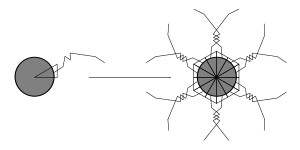
\includegraphics[width=0.45\textwidth]{diffuseSchreiberFig2}
  \end{center}
  \caption[]{\label{fig-schrieberFig12}
  (a) Motion in the fundamental domain (top left), elementary cell (top
      right) and the full space (bottom).
  (b) The above trajectory unwrapped in the full space and its 12 copies
    obtained by applying all point group \Dn{6} actions to it (from
    \refref{CGS92}).
  }
\end{figure}

When, in addition to translational invariance, the elementary cell is
invariant under a discrete symmetry group (point group) $G$, the lattice
can be tiled into images under $G$ and the lattice translations of a
fundamental domain.

The symmetry of the triangular periodic Lorentz gas is the space group
$p6mm$ (see Cotton\rf{Cotton08} {\em Chemical applications of group
theory},  Chapt.~11, for a pretty discussion of the geometry of space
groups). Space group $p6mm$ has a point subgroup $C_{6v}=\Dn{6}$. Leaving
the mathematical representation of group for later discussion, we can
intuitively understand the symmetry by decomposing the hexagonal
elementary cell into 12 identical triangular tiles, as in
\reffig{fig-schrieberFig12}\,(a), upper left, the fundamental domain and
its 11 copies. The fundamental domain tiles the full hexagon, by
application of the \Dn{6} rotations around the center or reflection along
symmetry lines, i.e. the point group actions.

In \refsect{s-Lorentz} we had reduced a trajectory from full space to
elementary cell, as in \reffig{fig-schrieberFig12}\,(a), upper right,
using the translational symmetry, and were able to compute various
quantities in terms of elementary cell \po s. In this section we will
further use the point group symmetry to derive the fully symmetry-reduced
trace formula and, for the first time, the diffusion constant using
cycles restricted to the fundamental domain.

As we will work with three kinds of \statesp s,
we state here what tildes, nothings and hats atop symbols signify:
\bea
\tilde{\ }     &~~&
    \mbox{fundamental domain, triangle in \reffig{fig-schrieberFig12}}
        \continue
%[nothing] \qquad \qquad &&
[0pt] \qquad \qquad &&
    \mbox{elementary cell, hexagon in \reffig{fig-schrieberFig12}}
        \continue
\hat{\ }   &&
    \mbox{full {\statesp}, lattice in \reffig{fig-schrieberFig12}}
\label{atops}
\eea
It is convenient to define an \evOper\ for each of the 3
cases of \reffig{fig-schrieberFig12}.
$\hx(t)\,=\,\hflow{t}{\hx}$
denotes the point in the global space
$\hM$
reached by the flow in time $t$.
$x(t)\,=\,\flow{t}{\xInit}$
denotes the corresponding flow in the elementary cell;
the two are related by
\beq
\hn_t(\xInit)= \hflow{t}{\xInit} - \flow{t}{\xInit} \in T
\,,
\ee{l-diff-hatn}
the translation of the endpoint of the global path into the elementary
cell $\pS$. The quantity $\tx(t)\,=\,\tflow{t}{\tx}$ denotes the flow in
the fundamental domain ${\widetilde \pS}$; $\tflow{t}{\tx}$ is related to
$\flow{t}{\tx}$ by a discrete symmetry $g \in G$ which maps
$\tx(t)\in {\widetilde \pS}$ to ${x}(t) \in {\pS}$.

Starting any point $\ssp$ on a elementary cell cycle $p$, after completing a cycle the particle crosses each cell boundary the same number of times. Because translations are commutative, the particle will always reach the same copy of elementary cell. By eq. \refeq{l-diff-hatn} the total displacement along the cycle is independent of the point of choice. In other words, the displacement is an invariant of the elementary cell cycle. However, when we take into account the point group symmetry (i.e. rotations and reflections), the above statement does not stand. We will need to address the non-commutativity of symmetries and develop new invariants to compute diffusion coefficient.

%\begin{figure}[htbp]
%  \begin{center}
%    (a)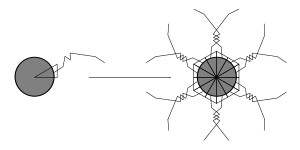
\includegraphics[width=0.45\textwidth]{diffuseSchreiberFig2}
%    (b)\includegraphics[width=0.45\textwidth]{diffuseSchreiberFig3}
%  \end{center}
%  \caption[]{ \label{fig:schrieberFig23} (a) An (unwrapped) trajectory (in full
%  space) and its 12 copies after applying point group actions to it. (b)
%  Multiplicity of periodic orbits in fundamental domain.}
%\end{figure}

%When the scattering array has a discrete symmetries, such as
%reflection symmetry, each elementary cell may be built from a {\em
%fundamental domain} ${\widetilde \pS}$ by the action of a discrete (not
%necessarily abelian) group $G$. The quantity $\tx(t)\,=\,\tflow{t}{\tx}$
%denotes the flow in the fundamental domain ${\widetilde \pS}$;
%$\tflow{t}{\tx}$ is related to$\flow{}{\tx}$ by a discrete symmetry $g
%\in G$ which maps $\tx(t)\in{\widetilde \pS}$ to ${x}(t) \in {\pS}$. The
%full $\hM \rightarrow {\widetilde\pS}$ reduction is complicated by the
%non-abelian nature of $G$, and will be illustrated in this section in
%detail.

\PC{2016-01-01}{explain that any elementary cycle point translate by the
same amount in the full {\statesp}}

\subsection{Point group changes translation \label{sec-point-group-translation}}

While a full space (or elementary cell) trajectory can be uniquely reduced to its fundamental domain counter part by wrapping (reflecting and rotating) all the individual segments in different fundamental domain into a single one, the reverse process is always one-to-many. Because the fundamental domain do not have the concepts of absolute orientation, a single unwrapped trajectory may have up-to 12 isometric copies after we apply the discrete group actions. Even worse, depending on where we start to unwrap the trajectory, the full space trajectories can be completely different in shape. A precise mathematical treatment is necessary to address the above effects, before we can proceed to the complete formula for diffusion, which depends on descriptions of displacements.

We start by first working on the relation of translation and discrete symmetry. A point $\ssp$ in the elementary cell is identified by its
fundamental domain mirror image:
\[ %beq
\ssp=g\,\tx,
\] %eeq
given a group action $g\in G$. We have to appreciate that both the full space flow $\hflow{t}{\ssp}$ and elementary flow $\flow{t}{\ssp} $ is G-equivariant under the lattice group symmetry,.
\[
\hflow{t}{g\,\tx} = g\,\hflow{t}{\tx}\,,
\flow{t}{g\,\tx} = g\,\flow{t}{\tx}
\]

Then the displacement in full space is also G-equivariant:
\[ %beq
\hn_t(\ssp)= \hflow{t}{g\,\tx} - \flow{t}{g\,\tx}=g\,(\hflow{t}{\tx} - \flow{t}{\tx}) = g\,\hn_t(\tx)\,.
\] %eeq

We apply this rule to the displacement associated with a prime
periodic orbit $\tp$ restricted in the fundamental domain.
Let $\tp\equiv\{\tx_0,\tx_1,\ldots,\tx_{\cl{\tp}}\}$, with topological length
$\cl{\tp}$ and $\tx_i$ the bouncing points on the orbit.


For each free flight (\eg, from $\tx_i$ to $\tx_{i+1}$) we denote the associated
displacement in full space $\hn(\tx_i,e)$. Special caution has to be
taken when we add the individual displacements together as the particle moves
along a fundamental domain orbit. Each time the particle crosses a boundary (which is the symmetry line), it is deflected back in the same domain as if it hits a wall.
However, in the elementary cell the particle has already entered another triangular copy, and we have to record the associated group action that can map it back. Before the next collision, we assign $g_\tp(\tx_{i+1},\tx_{i})$  as the total group element during the flight to keep track of changes in absolute orientation. We can now write the displacement traveled along the orbit, after finishing a full cycle:
\beq
\hn_{\tp}(\tx_{0})=\sum_{i=0}^{\cl{\tp}-1}\hn(\tx_{i},g_{\tp,\tx_0}(\tx_{i}))
=\sum_{i=0}^{\cl{\tp}-1}g_{\tp,\tx_{0}}(\tx_{i})\,\hn(\tx_{i},e),
\eeq
where $g_{\tp,\tx_{0}}(\tx_i)=\prod_0^{j-1} g_\tp(\tx_{j+1},\tx_{j})$ is
the accumulated orientation changes along the orbit when starting from
$\tx_{0}$. The displacement has an explicit dependence on starting point. We denote the total group action (orientation change) for the orbit
\bea
h_{\tp}(\tx_i)&\equiv& g_\tp(\tx_{i},\tx_{i-1})\,\ldots\,
g_\tp(\tx_{0},\tx_{\cl{\tp}-1})\nonumber\\
&& \, g_\tp(\tx_{\cl{\tp}-1},\tx_{\cl{\tp}-2})\, \ldots\,
g_\tp(\tx_{i+1},\tx_{i}),
\eea

which also immediately connects the flow in fundamental domain and elementary cell by
\[\flow{t_\tp}{\tx_i}=h_{\tp}(\tx_i)\tflow{t_\tp}{\tx_i}.\]

Although the group action $h_{\tp}(\tx_i)$ depends on the initial points
on the orbit as well, it is a property of the orbit's symmetry. One can easily show that all $h_{\tp}(\tx_i), \tx_i\in\tp$ belong to the \emph{same} subgroup of $G$.


If we let the particle (starting from $\tx_i$) travel along the fundamental domain orbit $r$ times, the cumulated displacement is then given by:
\beq
\hat{L}_{\tp}^{r}(\tx_i)\equiv
(e+\hp^{1}(\tx_i)+\cdots+\hp^{r-1}(\tx_i))\cdot\hn_{\tp}(\tx_i),
\label{eq-fdDisplacement}
\eeq


\subsection{Fundamental domain diffusion tensor}
\label{s-fundDiff}
  % fundDiff.tex      pdflatex ZhCvGo15
% Diffuse globally, compute locally: a cyclist tale
% Tingnan Zhang, Daniel I. Goldman and Predrag Cvitanovi\'c

%\subsection{Fundamental domain diffusion tensor}
%\label{s-fundDiff}

Previous literatures on discrete factorization: how it works for the
scalar quantities and why it does not work for the vector quantity such
like displacement.

We start from the trace trace of \evOper\ \refeq{eq-eOper} and project it
into the individual representations of the discrete group:
\bea
\tr{\cal L}^t &=& \sum_{\alpha \in\II_G} \tr{\cal L}_{\alpha}^t\nonumber\\
\tr{\cal L}_{\alpha}^{t} &=& \frac{d_\alpha}{|G|}\sum_{\sigma \in
  G}\sum_{h\in G}\chi_\alpha(h)\int_{\t {\cal M}} d\tx \delta (h\tx -
\flow{t}{\tx})e^{\beta\cdot\sigma\cdot\hn^t(\tx)}.\nonumber\\
\label{eq-traceSum}
\eea

The $\delta$-function part $\delta (h\tx - \flow{t}{\tx})$ in the integral
selects the fundamental domain periodic points that satisfy the group
condition $h\equiv h^r_{\tp}(\tx_i)$. The displacement traveled starting
from each of those points and along the orbit $r$ times takes the form
already computed in\refeq{eq-fdDisplacement}. The rest is straight
forward gymnastics of algebra,which yields the dynamical zeta function
for the $\alpha$ irreducible representation:
\begin{widetext}
 \beq
\frac{1}{\zeta_{\alpha}(\beta,s,z)}
=\exp\left(-\frac{d_\alpha}{|G|}\sum_{\sigma\in G}\sum_{\tp}
    \frac{1}{\cl{\tp}}\sum_{\tx_{i}\in\tp}\sum_{r=1}^{\infty}
    \frac{t_{\tp}^{r}}{r}
    \chi_{\alpha}(\hp^{r}(\tx_i))e^{\beta\cdot\sigma\cdot\hat{L}_{\tp}(r,\tx_i)}
    \right),
\label{eq-fdZeta}
\eeq
\end{widetext}

where
\[
  t_{\tp}\equiv
\frac{z^{\cl{\tp}}e^{-sT_{\tp}}}{|\ExpaEig_\tp|}
\,,
\]
is the weight associated to the orbit. Equation \refeq{eq-fdZeta}
differs from its counterpart in elementary cell, but can be reduced to if
the symmetry group contains only $e$.

We are interested in the one dimensional, symmetric trivial
representation with$ d_\alpha = 1 $ and all $ \chi(h) = 1 $; there by we
drop the subscript $\alpha $ in the following calculation. Partial
derivative with respect to$\beta$ gives:
\begin{widetext}
\bea
\frac{\partial^{2}}{\partial\beta^{2}}\frac{1}{\zeta(\beta,s,z)}
&=\frac{1}{\zeta(\beta,s,z)}\left(\left(\frac{1}{|G|}
\sum_{\sigma\in G}\sum_{\tp}\sum_{\tx_i\in \tp}
\sum_{r=1}^{\infty}\frac{\sigma\cdot \hat{L}_{\tp}^{r}(\tx_i)t_{\tp}^r
e^{\beta\cdot\sigma\cdot \hat{L}_{\tp}^{r}(\tx_i)}}{\cl{\tp}r}\right)^{2}
    \right.
    \nonumber\\
&\left.-\frac{1}{|G|}\sum_{\sigma\in G}\left(\sum_{\tp}\sum_{\tx_i\in
      \tp}\sum_{r=1}^{\infty}\frac{\vert \sigma\cdot
      \hat{L}_{\tp}^{r}(\tx_i)\vert^{2}t_{\tp}^{r}e^{\beta\cdot\sigma\cdot
        \hat{L}_{\tp}^{r}(\tx_i)}}{\cl{\tp}r}\right)\right).
        \eea
\end{widetext}
The first term in the formula corresponds to $ \langle\hx\rangle^2 $ and
second to $ \langle\hx^2\rangle $. It is trivial to see that
\beq\sum_{\sigma\in G}\frac{\sigma\cdot
  \hat{L}_{\tp}^r(\tx_i)t_{\tp}^r e^{\beta\cdot\sigma\cdot
  \hat{L}_{\tp}(r,\tx_i)}}{\cl{\tp}r} \equiv 0,
\eeq
because of the summation over the discrete group $\Group$. Thus the calculated
mean drift is zero, consistent with the symmetry of the system. Observing
that the length$\vert \sigma\cdot \hat{L}_{\tp}^{r}(\tx_i) \vert$ does
not change under rotation, we write
\bea
\langle\hx^2\rangle &=& \left.\frac{1}{\zeta(\beta,s,z)}\sum_{\tp}
\sum_{r=1}^{\infty}\frac{t_{\tp}^{r}}{r}
\sum_{\tx_i\in \tp}\frac{\vert\hat{L}_{\tp}^{r}(\tx_i)\vert^{2}}{\cl{\tp}}
    \right\vert_{\beta=0,s=0, z=1}
\nonumber\\
&=& \left.\prod_{\tp}\left(1-\frac{z^{\cl{\tp}}}{\vert\ExpaEig_\tp\vert
    }\right)\sum_{\tp}\sum_{r=1}^{\infty}\left(\frac{z^{\cl{\tp}}}{\vert\ExpaEig_\tp\vert
    }\right)^r\frac{\vert\hat{L}_{\tp}^{r}\vert^2}{r}\right\vert_{z=1}
\label{eq-meanSquareDisp}
\eea

with
\[
\vert\hat{L}_{\tp}^{r}\vert^2\equiv\sum_{\tx_i\in
  \tp}\frac{\vert\hat{L}_{\tp}^{r}(\tx_i)\vert^{2}}{\cl{\tp}}
\]
the average square displacement in full space when traveling along a fundamental
domain $r$ times. Formula \refeq{eq-meanSquareDisp} is an infinite polynomial in
the auxiliary variable $z$, and should be truncated to the topological length of
the longest periodic orbits find in calculation.


\subsection{Grammar of fundamental domain}
\label{s-fundGramm}
%  % fundGramm.tex      pdflatex ZhCvGo15
% Diffuse globally, compute locally: a cyclist tale
% Tingnan Zhang, Daniel I. Goldman and Predrag Cvitanovi\'c

% \subsection{Grammar of fundamental domain}
% \label{s-fundGramm}

\begin{figure}[htbp]
  \begin{center}
    (a) \includegraphics[width=0.35\textwidth]{diffuse7diskFundDflips}
    \\
    (b) \includegraphics[width=0.35\textwidth]{diffuse7diskFundDtiles}
  \end{center}
  \caption{\label{fig-7diskFundDflips}
  (a) Three generators tile the plane by flipping the fundamental domain
  across its three strait edges. Two are elements of \Dn{6}, the
  reflection  $s$ across the short disk-disk separation, and the
  reflection $\ell$ across the long disk-disk separation. Together they
  tile the elementary cell (hexagon in \reffig{fig-schrieberFig12}\,(a)
  upper right) by copies of the fundamental domain. Translations are
  generated by the reflection $f$ that pivots a  disk center to disk
  center by a flip across the symmetry line normal to the short disk-disk
  separation.
  (b) Tiling of the 7-disk by copies of the fundamental domain, labeled
  by a (not unique) sequence of the three generators  $\{s,\ell,f\}$,
  chosen so that each sequence contain one and only on  disk-to-disk
  pivot $f$.
  }
\end{figure}
    \TZ{2015-10-19}
    {I do not really use the three generators to compute the fundamental
    domain cycles, instead I use the idea of topological distinct flights
    (\reffig{fig-fdflights}). We have yet to discuss the equivalence
    between the 3-generators and topological distinct flight in the two
    figures.
    }
    \PC{2016-01-08}{Please always save the program that generated a given
    figure in \texttt{reducesymm/figSrc/} and document it in
    \texttt{reducesymm/figSrc/00ReadMe.txt}. Otherwise I have to degrade
    quality to split figures (as in \reffig{fig-fdflights}\,(c) and (b),
    and I have no way of editing labels.
    }

\begin{figure}[htbp]
  (a)\,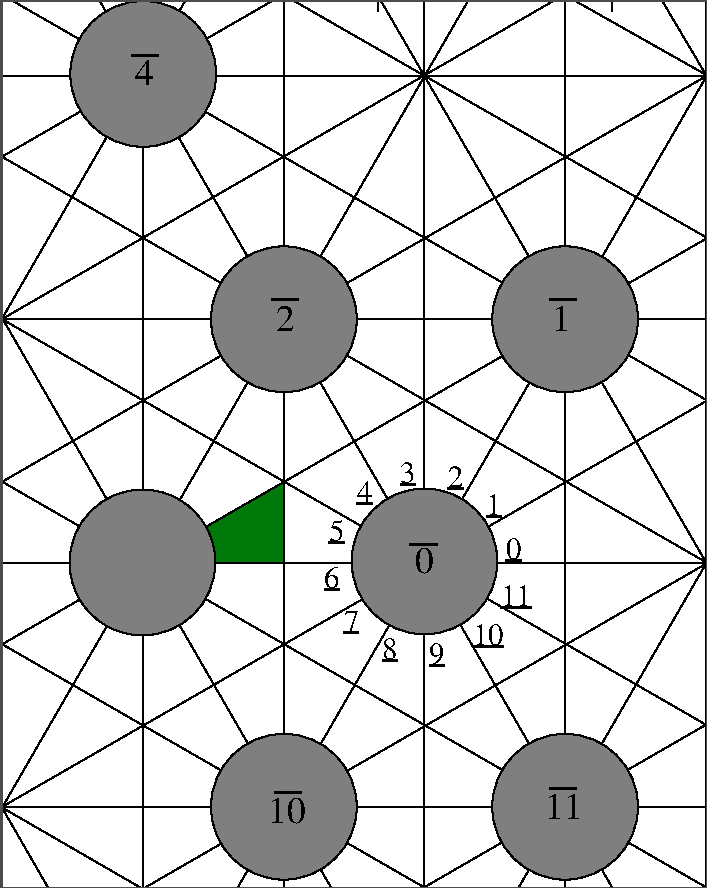
\includegraphics[width=0.35\textwidth]{diffuseFDSymbolIllustration}
  (b)\,\includegraphics[width=0.35\textwidth]{diffuseFDSymbolOrbits-b}
  (c)\,\includegraphics[width=0.35\textwidth]{diffuseFDSymbolOrbits-c}
  \caption{\label{fig-fdflights}
  Fundamental domain symbolic dynamics.
  (a) With  imposed finite horizon and starting on the edge of a disk in
  fundamental  domain (the green filled region), there are at most 6
  disks that can be reached by free flight (disks
  $\overline{0},\overline{1},\overline{2},\overline{4},\overline{10}$ and
  $\overline{11}$).
  % Similar to how elementary cell symbolic dynamics are created,
  The reflection symmetry axes partition the circumference of
  a disk into 12 segments which we
  label counterclockwise, from $\underline{0}$ to $\underline{11}$. 
  (b) The fundamental domain fixed point
  $\{\overline{2},\underline{10}\}$, which corresponds to a periodic
  orbit of length 6 in elementary cell ($\cycle{0246810}$), is unwrapped
  in   global space. After each collision we re-label the disks and
  triangular   partitions according to their relative positions to the
  ``new'' fundamental   domain. In the figure labels are also rotated
  according to the point   group actions.
  }
\end{figure}


%In the international crystallographic notation, the hexagonal lattice is
%called $p6mm$, with point group $6mm$, where prefix $p$ indicates that
%the unit cell is primitive (not centered),

Existing elementary cell symbolic dynamics cannot generate the prime fundamental domain orbits. While the 12 symbols partition the elementary cell state space into distinct regions, when wrapped into the fundamental domain state space, the regions begin to overlap. Thus, we developed a new symbolic description to numerically compute the cycles in the fundamental domain, by means of tile generators, which we quantify now. 

Tracking an arbitrary trajectory in the fundamental domain, we can distinguish two types of bounces: those on the disk edge and on one of the symmetry lines. As discussed in \ref{sec-point-group-translation}, the latter will add group operations on the trajectory. We enumerate all the elements in the point group $C_{6v}$:

\beq
\Group = \{
e, C_6^+, C_6^-, C_3^+, C_3^-, C_2,
\sigma_{d1}, \sigma_{d2}, \sigma_{d3},
\sigma_{v1},\sigma_{v2}, \sigma_{v3}
\}
\,,
\eeq
with $s=\sigma_{d}$ the reflection across the short disk-disk separation,
and $\ell=\sigma_{v}$ reflection across the long disk-disk separation
generators of \Dn{6}. The entire space group $p6mm$ is then generated by
adding a disk-to-disk generator $f$ that pivots a disk center to another
by flip across the symmetry line normal to the short disk-disk
separation, \reffig{fig-7diskFundDflips}\,(a). We find it convenient to
define $C$ as the generator of cyclic rotations by $\pi/3$,
\beq
\ell s = C_6^- = C
\,,\quad
C^6 = e
\,;\qquad
s \ell =  C_6^+
\,,\qquad
s  =  C_6^+ \ell
\,.
\eeq
    \TZ{2015-10-22}
    {The idea is that the topological periodic orbit in the fundamental
    domain is not sensitive to the order of flips. When $w$ increases,
    one might notice that a single flight along the orbit changes from
    $sf$ to $fs$. However, the relative position between the start and
    end triangular cells are always the same.}

A free flight between two disks in the full space may then be wrapped into
fundamental domain, according to the sequence of edges $\{s,\ell,f\}$ it
passed. There are many different paths when jump to the nearest disk: it can be
as simple as a single pivot $f$, or can be more complex such like $\ell f s$
that involves crossing multiple symmetry lines,
~\reffig{fig-7diskFundDflips}\,(b). We also notice that some symbol combinations
are topologically equivalent, in the sense that they yield the same group
actions. For example, the short jump $sf$ is topologically equivalent to $fs$,
because the particle ends up in the same copy of fundamental domain before the
next collision.

Our next task is to generate all topologically distinct itineraries from $\{s,\ell,f\}$. We can immediately realize a partial list of the equivalence relations:
\bea
f s &=& s f
\,,\nonumber\\
f \ell f&=&\ell f \ell
\,.
\eea
All longer equivalence relations in ~\reffig{fig-7diskFundDflips} can be
reduced to the above primitive ones:
\bea
f s \ell &=& s f \ell\,,\nonumber\\
\ell f\ell s &=& f \ell s f\,.
\eea

There are also some pruning rules to keep in mind. Because a free flight
cannot cross the same border twice, sequences including $\ell\ell,ff,ss$
are forbidden. $C^3$ (and all higher orders) is also pruned as the
particle cannot cross the center hard disk; nor swirl around it.

While the string description of flight is mathematically rigorous, it is
practically impossible to be encoded into programs for computing the orbits,
because the number of equivalent strings increases exponentially when the length
of the orbit (and also the string) increases. However, there is a more
physically intuitive way to organize the symbols, by means of ``topological
flight'', \reffig{fig-fdflights}\,(a). In this representation, a equivalence
relation like $sf\equiv fs$ can be uniquely identified by a combination of a
disk number and a partition number $\{\overline{0},\underline{6}\}$. Longer
flight such like $\ell f \ell s \ell f \equiv  f \ell f s \ell f \equiv f \ell s
f \ell f \equiv f \ell s \ell f \ell$ that cross many boundaries now yields a
very simple symbol pair $\{\overline{1},\underline{5}\}$. 

Because this compact representation only takes into consideration the starting
and ending points of a free flight, the exponentially long list of equivalent
strings are eliminated. The topological flight leads to a straight forward
numerical scheme to find cycles. The disk number fixes the two ends of the free
flight while the partition number limits the range of angles on the disk.
Similar to searching cycles in the elementary cell, we now have a constrained
version of convex minimization problem which can be solved using standard
non-linear optimization approach.



 \TZ{2015-11-02}
    {I have not yet talked about the pruning rule in detail here; it is
    more complicated bases on the reflection angle}


\begin{figure}[htbp]
  \begin{center}
    (a) \includegraphics[width=0.35\textwidth]{diffuse7diskFundDflips}
    (b) \includegraphics[width=0.35\textwidth]{diffuse7diskFundDtiles}
  \end{center}
  \caption{\label{fig-7diskFundDflips}
  (a) The three generators of tiling of the  plane by a fundamental
  domain: two generators of \Dn{12} tiling, reflection  $s$ across the
  short disk-disk separation, reflection $\ell$ across the long
  disk-disk separation; and a translation generator $f$ that pivots
  (`flips') a  disk center to disk center by flip across the symmetry
  line normal to the short disk-disk separation.
  (b) Tiling of the 7-disk by copies of the fundamental domain, labeled
  by a (not unique) sequence of the three generators  $\{s,\ell,f\}$,
  chosen so that each sequence contain one and only on  disk-to-disk
  pivot $f$.
  }
\end{figure}
    \TZ{2015-10-19}
    {I do not really use the three generators to compute the fundamental
    domain cycles, instead I use the idea of topological distinct flights
    (\reffig{fig-fdflights}). We have yet to discuss the equivalence
    between the 3-generators and topological distinct flight in the two
    figures. }

\begin{figure}[htbp]
  (a)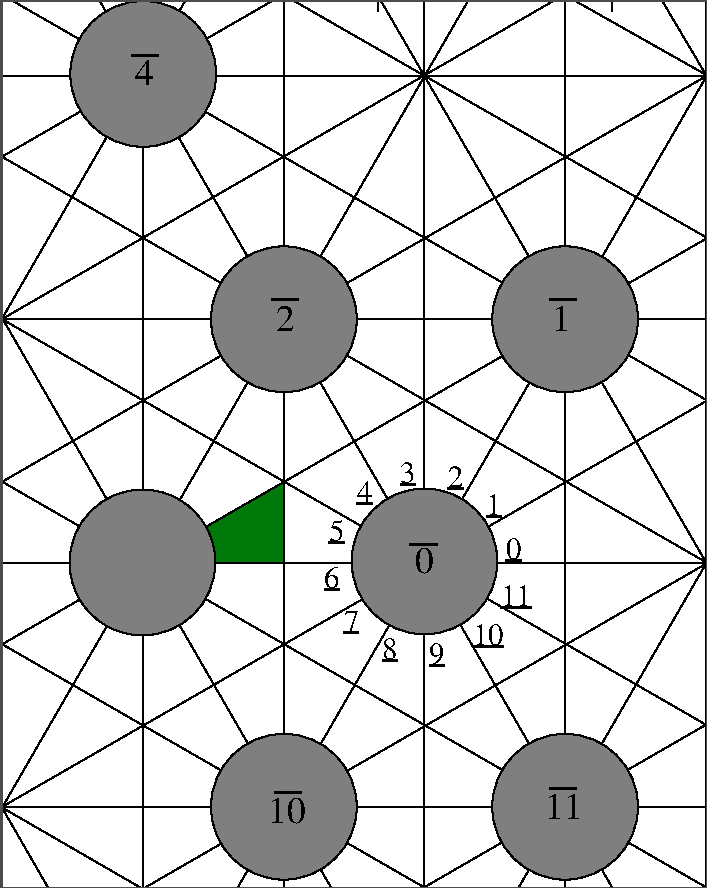
\includegraphics[width=0.35\textwidth]{diffuseFDSymbolIllustration}
  (b)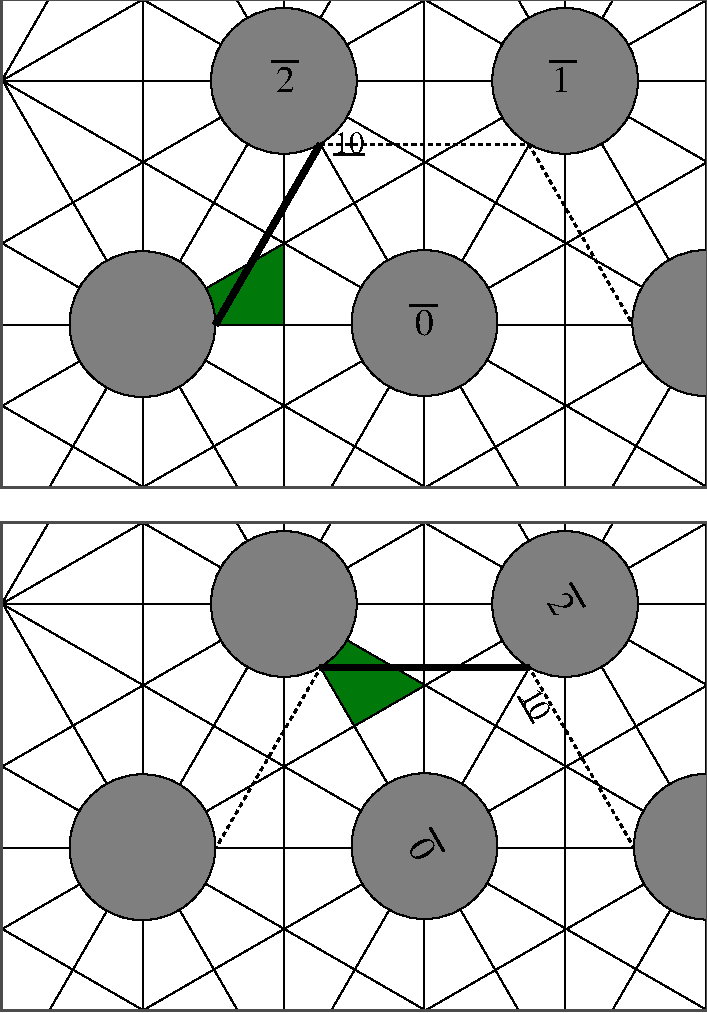
\includegraphics[width=0.35\textwidth]{diffuseFDSymbolOrbits}
  \caption{\label{fig-fdflights}
  Fundamental domain symbolic dynamics.
  (a) With  imposed finite horizon and starting on the edge of a disk in
  fundamental  domain (the green filled region), there are at most 6
  disks can be reached  without collision (disk
  $\overline{0},\overline{1},\overline{2},\overline{4},\overline{10}$ and
  $\overline{11}$). Similar to how elementary cell symbolic dynamics are
  created, we label the 12 triangular pieces of a disk in a counter
  clock-wise  manner, from $\underline{0}$ to $\underline{11}$. The
  combination of a disk  label and a triangular piece label
  $\{\overline{i},\underline{j}\}$ uniquely  identifies a topologically
  distinct flight.
  (b) The fundamental domain fixed point
  $\{\overline{2},\underline{10}\}$, which corresponds to a periodic
  orbit of length 6 in elementary cell ($\cycle{0246810}$), is unwrapped
  in   global space. After each collision we re-label the disks and
  triangular   partitions according to their relative positions to the
  ``new'' fundamental   domain. In the figure labels are also rotated
  according to the point   group actions.
  }
\end{figure}



In the international crystallographic notation, the hexagonal lattice is
called $p6mm$, with point group $6mm$, where prefix $p$ indicates that
the unit cell is primitive (not centered),
\beq
\Group = \{
e, C_6^+, C_6^-, C_3^+, C_3^-, C_2,
\sigma_{d1}, \sigma_{d2}, \sigma_{d3},
\sigma_{v1},\sigma_{v2}, \sigma_{v3}
\}
\,,
\eeq
with $s=\sigma_{d}$ the reflection across the short disk-disk separation,
and $\ell=\sigma_{v}$ reflection across the long disk-disk separation
generators of \Dn{12}. The entire space group $p6mm$ is then generated by
adding a disk-to-disk generator $f$ that pivots a disk center to another
by flip across the symmetry line normal to the short disk-disk
separation, \reffig{fig-7diskFundDflips}a. We find it convenient to
define $C$ as the generator of cyclic rotations by $\pi/3$,
\beq
\ell s = C_6^- = C
\,,\quad
C^6 = e
\,;\qquad
s \ell =  C_6^+
\,,\qquad
s  =  C_6^+ \ell
\,.
\eeq
    \TZ{2015-10-22}
    {The idea is that the topological periodic orbit in the fundamental
    domain is not sensitive to the order of flips. When $w$ increases,
    one might notice that a single flight along the orbit changes from
    $sf$ to $fs$. However, the relative position between the start and
    end triangular cells are always the same.}
A free flight between two disks in the full space may then be wrapped
into fundamental domain, according to the sequence cell edges
$\{s,\ell,f\}$ it passed. For example, there are different paths when
jump to disk $0$: it can be as simple as a single pivot about $f$, or can
be more complex such like $\ell f s$ that involves multiple flips,
~\reffig{fig-7diskFundDflips} b. Although we can associate each free
flight with a chain of the generators, some of the combinations are
equivalent. The short jump $sf$ is topologically equivalent to $fs$, in
the sense that the particle ends up in the same copy of fundamental
domain before next collision.

Our task is to generate all distinct itineraries from $\{s,\ell,f\}$. One
can immediately realize a partial list of the equivalence relations:
\bea
f s &=& s f
\,,\nonumber\\
f \ell f&=&\ell f \ell
\,.
\eea
All longer equivalence relations in ~\reffig{fig-7diskFundDflips} can be
reduced to the above primitive ones:
\bea
f s \ell &=& s f \ell\,,\nonumber\\
\ell f\ell s &=& f \ell s f\,.
\eea

There are also some pruning rules to keep in mind. Because a free flight
cannot cross the same border twice, sequences including $\ell\ell,ff,ss$
are forbidden. $C^3$ (and all higher orders) is also pruned as the
particle cannot cross the center hard disk; nor swirl around it.

While the string description of flight is mathematically rigorous and
accurate, it is practically hard to be encoded into programs for
computing the orbits, because the number of equivalent strings increases
exponentially when the length (of a single string) increases. However,
there is a more physically intuitive way to organize the type of flight,
by means of ``topological flight'', \reffig{fig-fdflights} (a). In this
representation, a equivalence relation like $sf\equiv fs$ can be uniquely
identified by a combination of a disk number and a partition number
$\{\overline{0},\underline{6}\}$. Longer flight such like $\ell f \ell s
\ell f \equiv  f \ell f s \ell f \equiv f \ell s f \ell f \equiv f \ell s
\ell f \ell$ that cross many boundaries now yields a very simple symbol
pair $\{\overline{1},\underline{5}\}$.

The topological flight leads to a straight forward numerical scheme to
find cycles. The disk number fixes the two ends of the free flight while
the partition number limits the range of angles on the disk. Similar to
searching cycles in elementary cell, we now have a constrained version of
numerical minimization problem which can be solved using standard
non-linear optimization approach.
 \TZ{2015-11-02}
    {I have not yet talked about the pruning rule in detail here; it is
    more complicated bases on the reflection angle}

\subsection{Diffusion in the fundamental domain}
\begin{table}[htbp]
\hfill
\TZ{2015-10-19}{Do we need this many digits in the table?}
\begin{tabular}{|r|r|r|l|l|}
\hline
$\period{p}$ & \# cycles & $\zeta$(0,0) & $\lambda$ & D \\ \hline\hline
1      & 5      & -0.2169759 & 1.39193 & 0.37795 \\
2      & 10     & -0.0248233 & 1.74541 & 0.23118\\
3      & 33     & -0.0221962 & 1.72235 & 0.25257\\
4      & 108    & -0.0002192 & 1.74450 & 0.24165\\
5      & 373    &  0.0023463 & 1.76079 & 0.24468\\
6      & 1378   &  0.0096330 & 1.75610 & 0.24068\\ \hline\hline
\multicolumn{3}{|l|}{numerical experiment}
                           & 1.760 & 0.25
\\ \hline
\end{tabular}

\caption{\label{TCELL2}
  Results for $w$=0.3. Calculation in FD. Gaspard 1992
  note: ``My numerical estimate for the Lyapunov exponent when $w=0.3$ is
  $\lambda = 1.760 \pm 0.002$, which supports the result of this table.''
}
\end{table}

\begin{figure}[htbp]
  \includegraphics[width=0.45\textwidth]{diffuseCycleExpansionResults}
  \caption[]{\label{fig-convergence}
  The convergence of diffusion coefficients  calculated using cycle
  expansion in elementary cell (green squares),  fundamental
  domain(orange squares). We  also show the convergence of ``periodic
  orbit expansion'' method, with and  without Shanks transformation
  (circles and diamonds) discussed in  \refref{Morriss1994}. Here $w = 0.3$.
  }
\end{figure}

\begin{figure}
\includegraphics[width=0.45\textwidth]{diffuseDiffCoefPlot}
  \caption[]{\label{fig-results} Diffusion coefficients as a function $w$.  Figure generated using data from various resources. Diamonds are results from  Green-Kubo numerical experiments\rf{MacZwa83}; stars\rf{BaEvCo93} and  circles\rf{GasBar95} are calculated from escape rate; and triangles are  given by Hausdorff fractal dimension calculation\rf{GasBar95}; dashed line  is a statistical approximation\rf{Angstmann20121819}}.
\end{figure}

       \TZ{2015-10-19}{Any comment on caption of \reffig{fig-convergence}?}
Compared with various methods, the symmetry reduced cycle expansion
method converges the fastest, table \ref{TCELL2} and
\reffig{fig-convergence}. Diffusion coefficient computed from $\sim2000$
fundamental domain cycles of topological length up to 6 gives two
significant digits, while the elementary cell calculation needs over
$\sim 10000$ cycles in order to converge. In other words, the fundamental
domain cycles suggests a better and denser partition of the phase space.
    \TZ{2015-10-19}{Talk about other two methods}.

To further test \refeq{eq-meanSquareDisp}, we compute the diffusion
coefficient for $w/r = 0.05, 0.10, 0.15, 0.20, 0.25, 0.30$, and compare
the results with existing numerical experiments and a recent statistical
estimation, \reffig{fig-results}. In Green-Kubol velocity
auto-correlation method the  diffusion coefficient can be extrapolated to
the accurate reference value $0.250$ (at $w/r=0.30$), using ensembles of
$10^6\sim10^7$ gas particles flying for long time $T>20$ (and the number
of bounces is greater than this)\rf{MacZwa83}. On the other hand, while
statistical approach yields a smooth analytical
formula\rf{Angstmann20121819}, the diffusion property is fundamentally
never a smooth, monotonically increasing function of $w$
    \TZ{2015-11-02}
    {what is that 1D diffusion reference that shows the anywhere
    continuous, nowhere smooth curve?}
Again, the effectiveness (yet correctness) of the cycle expansion is
proved by those comparison.

\section{Conclusion}
\label{s-concl}
  % siminos/froehlich/slice/concl.tex  called by FrCv11.tex
% $Author: predrag $ $Date: 2010-11-17 08:30:53 -0500 (Wed, 17 Nov 2010) $

% \section{Conclusion}

Many systems in fluid dynamics exhibit a continuous symmetry. Systems
such as the \KS\ flow\rf{ku,siv},
{\pCf}\rf{Visw07b,GHCW07,HGC08,HalcrowThesis}, and flow through an
cylindrical pipe\rf{Wk04,Kerswell05} demonstrate a simple product of
$\SOn{2}$ symmetries.

In this paper we have investigated using linear subspaces in
\mslices\ to replace a dynamical system with an equivalent
lower dimensional system. The two main obstacles to using the \mslices\
are that every point must be rotatable into the subspace and it can
introduce singularities into the flow. Locally linear slices are
guaranteed to intersect each group orbit only once, but it was shown that
linear slices will intersect every group orbit of a compact Lie group in
the {\statesp}, though it will do so multiple times. The \mslices\ can
introduce singularities into the flow that did not exist in the full
space. We demonstrated that as long as the group action is well behaved
(which it is for any general $\SOn{2}$ symmetry) then a trajectory
passing through a singularity corresponds to a simple shift in the
trajectory and does not cause any difficulties. In addition we
demonstrated that the problem of dealing with singularities of a product
of $\SOn{2}$ groups acting on different coordinates of the {\statesp}
(as is the case for the \KS\rf{ku,siv},
{\pCf}\rf{Visw07b,GHCW07,HGC08,HalcrowThesis}, and
pipe flows\rf{Wk04,Kerswell05}) is equivalent to dealing with the
symmetries of each \SOn{2}\ symmetry independently.



Even every slice cuts all group orbits, it makes no sense physically to
use one slice
(a set of all group orbit points that are closest to a given `template')
globally. Instead we should do what we already do for KS Poincar\'e sections.
We need to make a global chart by deploying both linear slices and linear
Poincar\'e sections in neighborhoods of the most important (relative)
equilibria and/or (relative) periodic orbits (those are tricky, because
slice fixing points must lie in the full \statesp, and have no symmetry,
so most of the solutions we have are not good as they stand). This is the
periodic-orbit generalization of the idea of
\HREF{http://chaosbook.org/overheads/trace/Tesselate.jpg}{\statesp\ tessellation}
so dear to professional cyclist(s).


Boundaries
between hyperplanes are themselves hyperplanes of one dimension less and
should be easy compute once we have decided on the set of slices. To find
what slice a given full \statesp\ trajectory point is in, one rotates
with respect to each slice, and checks whether the given group orbit
belong to it. In the \reducedsp\ the trajectory is integrated within a
given slice until it hits a hyperplane boundary - then one switches to
the next slice across the boundary. Boundary corners are measure zero, no
way you would hit them.

Global chart should be sufficiently fine-grained that we never hit any
slice singularities. That means that the neighborhood - bounded by
intersections with neighboring slices is sufficiently small that group
tangent space is nowhere within the slice - works in smooth flows
for sufficiently small neighborhoods.


More has to be done to reduce a system with a discrete
symmetry before the \mslices\ can be used for the continuous symmetry.


\begin{acknowledgments}
We are grateful to Pavel M. Svetlichnyy for many fruitful discussions in
the early stages of this project, and the key suggestion that the plane
can be tiled in terms of three elementary tiling generators.
TZ was supported by NSF grant ???-?????.
PC thanks to the family of late G. Robinson, Jr. and NSF grant
DMS-1211827 for partial financial support.
\end{acknowledgments}


% Choosing a journal automatically selects the correct APS BibTeX style
% file (bst file), so only uncomment the line below if necessary.
% \bibliographystyle{apsrev4-1}
% PC 2016-01-01  switched from siminos.bib to ChaosBook.bib
\bibliography{../bibtex/ChaosBook,../bibtex/diffuse}

\ifboyscout
% switch to Private
\eject %\newpage
    % reducesymm/tingnan/flotsam.tex    master file: diffuse/main.tex

\section{ZhCvGo15 flotsam}
\label{s:flotsam}

Squirrel away here potentially recyclable text from the
paper\rf{ZhCvGo15} proper, \texttt{diffuse/ZhCvGo15.tex}

%remember to cite Cvitanovi\'c and Eckhardt\rf{CvitaEckardt} {\em Symmetry
%decomposition of chaotic dynamics}

%A test of hyperlinking: what looks better?
%
%DasBuch\rf{DasBuch}
%or
%\refref{DasBuchMirror} {Chapter ``{World} in a mirror''}
%or trace~\refref{CBtrace}
%or \refref{Froeh10}
%or ChaosBook convergence\rf{CBconverg}
%or Predrag\rf{Cvi07}

As a billiard built up completely of concave surfaces and as a pure
hyperbolic system, the Lorentz gas is a good candidate for description in
terms of cycle expansions\rf{AACI}.

                                                            \toCB
\refRef{solomon1994chaotic} {\em Chaotic advection in a two-dimensional
flow: L\'evy flights and anomalous diffusion} studies chaotic transport
experimentally passive tracers in $2$\dmn\ rotating in laminar, chaotic,
and turbulent flows which can be described as anomolous deterministic
diffusion in periodic arrays. We do not touch that here.


%
%%%%%%%%%%%%%%%%%%%%%%%%%%%%%%%%%%%%%%%%%%%%%%%%%%%%%%%%%%%%%%%%%%
%\SFIG{fig_lor_4}
%{}{
%Deterministic diffusion in a
%finite horizon periodic Lorentz gas.
%\hfill (T. Schreiber)
%}{fig-lor-4}
%%%%%%%%%%%%%%%%%%%%%%%%%%%%%%%%%%%%%%%%%%%%%%%%%%%%%%%%%%%%%%%%%%
%

As a gedanken experiment, suppose a passively controlled robot is moving
in a boulder field at constant speed. The diffusion coefficient, which
describes roughly how much area the robot explored in a unit time, is the
key quantity we would like to investigate. We place the boulder in a
regular, periodic array and assume that we are in the heavy boulder limit
such that after each collision event, only the robot is deflected and
boulders remain immobilized. With the presumptions we effectively created
a periodic Lorentz gas model\rf{Dettm14} for locomotion in a boulder
field.

In biological field,  many important dynamical processes (often at
cellular level) are described in  terms of diffusion coefficients. Such
examples include the transport of ions  across the cell
membranes\rf{Stein12} and the movement of  microorganism(e.g.
bacterials) through natural  ecosystems\rf{koch1990diffusion}. In this
paper we will discuss the transport  property of more "macroscopic"
systems (such as moving  robots\rf{saranli2001rhex}) where a ``diffusive
description'' also applies.

Chaotic motions exist in many field of physics systems, blah. There are
physical problems such as beam defocusing in particle accelerators or
chaotic behavior of passive tracers in $2$\dmn\ rotating flows which can
be described as deterministic diffusion in periodic arrays. In the field
of animal/robotic locomotion, we will show that a macroscopic ``diffusion
view'' also applies.

In the macroscopic world, there are recent
studies shown that robotic locomotion in heterogeneous granular
environment also demonstrates scattering-diffusive pattern.

Lately, there has been an increased focus on robot locomotion in complex
environments (check Science and ROPP reference, the systematic study of
interactions between environment and locomotion, which we now
call``robophysics''). Many of those studies use substrates that are
spatially homogeneous and we have a good
understanding\rf{li2009sensitive,li2013terradynamics}. However, little is
known for locomotion in heterogeneous environment. There are some limited
experimental/theoretical studies for relatively simple settings (e.g.
slopes,ref). In this paper we intend to approach the longterm transport
properties of locomotion in a more complex environment, i.e. in a field
of scatterers of which the scales are comparable to the locomotor.

% \newpage
\fi


\end{document}



% If in two-column mode, this environment will change to single-column
% format so that long equations can be displayed. Use sparingly.
% \begin{widetext}
%   put long equation here
% \end{widetext}

% Use the figure* environment if the figure should span
% across the entire page. There is no need to do explicit centering.

% Surround figure environment with turnpage environment for landscape
% figure
% \begin{turnpage}
%   \begin{figure}
%     \includegraphics{}%
%     \caption{\label{}}
%   \end{figure}
% \end{turnpage}

% Here is an example of the general form of a table:
% Insert the column specifiers (l, r, c, d, etc.) in the empty braces of the
% \begin{tabular}{} command.  The ruledtabular enviroment adds doubled
%   rules to table and sets a reasonable default table settings.  Use
%   the table* environment to get a full-width table in two-column Add
%   \usepackage{longtable} and the longtable (or longtable*}
%   environment for nicely formatted long tables. Or use the the [H]
%   placement option to break a long table (with less control than in
%   longtable).
% \begin{table}%[H] add [H] placement to break table across pages
% \caption{\label{}}
% \begin{ruledtabular}
%   \begin{tabular}{}
% Lines of table here ending with \\
% \end{tabular}
% \end{ruledtabular}
% \end{table}

% Surround table environment with turnpage environment for landscape
% table
% \begin{turnpage}
%   \begin{table}
% \caption{\label{}}
% \begin{ruledtabular}
%   \begin{tabular}{}
% \end{tabular}
% \end{ruledtabular}
% \end{table}
% \end{turnpage}
